\documentclass[10pt,a4paper]{article}

% ------------------------------------------------------------------
% Cours de préparation --- Ce que voit un détecteur de musique IA
% Compilation : pdflatex (2 passes) ou latexmk -pdf
% ------------------------------------------------------------------
\usepackage[utf8]{inputenc}
\usepackage[T1]{fontenc}
\usepackage{lmodern}
\usepackage[french]{babel}
\usepackage[a4paper,left=2.1cm,right=2.1cm,top=2.2cm,bottom=2.1cm]{geometry}
\usepackage{microtype}
\usepackage{amsmath,amssymb,mathtools,bm}
\usepackage{array,booktabs,tabularx,enumitem}
\usepackage{xcolor}
\usepackage{fancyhdr}
\usepackage{titlesec}
\usepackage{listings}
\usepackage{graphicx}
\usepackage{multicol}
\usepackage{caption}
\usepackage[skins,breakable]{tcolorbox}
\usepackage{tikz}
\usetikzlibrary{arrows.meta,babel,calc}
\usepackage[colorlinks=true,linkcolor=blue!50!black,urlcolor=blue!50!black,citecolor=blue!50!black]{hyperref}

\linespread{1.02}
\setlength{\parindent}{0pt}
\setlength{\parskip}{3.5pt}
\setlength{\headheight}{13pt}
\setlist[itemize]{leftmargin=1.3em,itemsep=1pt,topsep=2pt,parsep=0pt}
\setlist[enumerate]{leftmargin=1.6em,itemsep=1pt,topsep=2pt,parsep=0pt}
\setlength{\topsep}{2pt}
\captionsetup{font=small,labelfont=bf,skip=3pt}
\setlength{\textfloatsep}{8pt plus 2pt minus 2pt}
\setlength{\floatsep}{6pt plus 2pt minus 2pt}
\setlength{\intextsep}{6pt plus 2pt minus 2pt}
\renewcommand{\topfraction}{0.9}
\renewcommand{\floatpagefraction}{0.8}
\newcolumntype{L}[1]{>{\raggedright\arraybackslash}p{#1}}

\titleformat{\section}{\Large\bfseries}{\thesection}{0.6em}{}
\titleformat{\subsection}{\large\bfseries}{\thesubsection}{0.5em}{}
\titlespacing*{\section}{0pt}{12pt plus 2pt}{4pt}
\titlespacing*{\subsection}{0pt}{8pt plus 2pt}{2pt}

\pagestyle{fancy}
\fancyhf{}
\renewcommand{\headrulewidth}{0.3pt}
\fancyhead[L]{\small Cours de préparation --- détection de musique IA}
\fancyhead[R]{\small 7 novembre 2026}
\fancyfoot[C]{\small\thepage}

% --- macros ---
\newcommand{\sV}{\textsuperscript{\scriptsize\textcolor{green!40!black}{[V]}}}
\newcommand{\sR}{\textsuperscript{\scriptsize\textcolor{orange!80!black}{[R]}}}
\newcommand{\sM}{\textsuperscript{\scriptsize\textcolor{red!70!black}{[M]}}}
\newcommand{\sN}{\textsuperscript{\scriptsize\textcolor{black!60}{[N]}}}
\newcommand{\tprfpr}{\mathrm{TPR}@1\,\%\mathrm{FPR}}
\newcommand{\AUC}{\mathrm{AUC}}
\newcommand{\EER}{\mathrm{EER}}
\newcommand{\TPR}{\mathrm{TPR}}
\newcommand{\FPR}{\mathrm{FPR}}
\newcommand{\hyp}[1]{\textit{(hypothèse du projet : #1)}}
\newcommand{\nref}[1]{\textsuperscript{\scriptsize\textcolor{black!55}{#1}}}

\newtcolorbox{retenir}[1][À retenir]{enhanced,colback=blue!3!white,colframe=blue!45!black,
  boxrule=0.5pt,arc=2pt,left=5pt,right=5pt,top=3pt,bottom=3pt,
  fonttitle=\bfseries\small,title={#1},before skip=5pt,after skip=5pt,breakable}
\newtcolorbox{projet}{enhanced,colback=orange!6!white,colframe=orange!60!black,
  boxrule=0.5pt,arc=2pt,left=5pt,right=5pt,top=3pt,bottom=3pt,
  fonttitle=\bfseries\small,title={Lien avec le projet},before skip=5pt,after skip=5pt,breakable}

\lstset{basicstyle=\ttfamily\scriptsize,frame=single,rulecolor=\color{black!30},
  backgroundcolor=\color{black!3},aboveskip=4pt,belowskip=4pt,xleftmargin=2pt,xrightmargin=2pt,
  columns=fullflexible,keepspaces=true,showstringspaces=false,
  commentstyle=\color{green!35!black},keywordstyle=\color{blue!60!black}}

\hypersetup{pdftitle={Cours de préparation --- Ce que voit un détecteur de musique IA}}

\begin{document}

% ------------------------------------------------------------------
\begin{center}
{\large\scshape Cours de préparation au projet}\\[0.3em]
{\LARGE\bfseries Ce que voit un détecteur de musique IA}\\[0.3em]
{\normalsize Signal audio, codecs et générateurs neuronaux, artefacts, détection, évaluation --- ce qu'il faut maîtriser pour réaliser le projet}
\end{center}

\begin{tcolorbox}[enhanced,colback=black!3!white,colframe=black!35,boxrule=0.4pt,arc=2pt,left=6pt,right=6pt,top=3pt,bottom=3pt,breakable]
\textbf{Mode d'emploi.} Ce cours remplace les cours de notions N1--N27 du dossier : il se lit dans l'ordre (environ 8\,h de lecture, exercices compris, estimation personnelle ; laboratoires L1--L9 hors lecture, résumés en annexe~C). Il suppose un niveau M2~IA (CNN, Transformers, PyTorch, ROC) et \emph{aucun} cours d'audio. Chaque notion porte son identifiant (\nref{N12}) pour retrouver le dossier. Ce qui vient d'un article est présenté comme \emph{établi par l'article} ; ce qui est une conjecture du projet est signalé \hyp{ainsi}.

\textbf{Statut des faits.} Les étiquettes suivent la convention du dossier :
\sV{} page ou article ouvert pendant la préparation de ce cours (mais lu par extraction automatique du texte : \emph{relire le PDF avant de citer un chiffre}) ;
\sR{} extrait de recherche, résumé ou fiche de dépôt, article non lu en entier ;
\sM{} connaissance générale non revérifiée, à contrôler avant de s'y fier ;
\sN{} source non ouverte (page refusée, vidéo, accès restreint).
Sans étiquette : calcul ou raisonnement donné dans le cours, que vous pouvez refaire. Les points à revérifier sont regroupés en annexe~D.
\end{tcolorbox}

\begin{center}\small
\begin{tabularx}{\textwidth}{@{}l X l r@{}}
\toprule
\textbf{Section} & \textbf{Notions du dossier} & \textbf{Semaine du projet} & \textbf{Page}\\
\midrule
\ref{sec:etat}\ État de l'art & N17, N18, N19 (cadre), N24 & avant la semaine~1 & \pageref{sec:etat}\\
\ref{sec:signal}\ Signal audio & N1, N2, N3, N4, N5 & phase~0, semaine~1 & \pageref{sec:signal}\\
\ref{sec:chaine}\ Chaîne commune et raccourcis & N19, N20, N27 & semaines 1--2 & \pageref{sec:chaine}\\
\ref{sec:eval}\ Apprentissage et évaluation & N6, N7, N8, N9, N26 & semaine~3 & \pageref{sec:eval}\\
\ref{sec:gen}\ Génération audio neuronale & N10--N16, N25, N12 & semaines 1--2 & \pageref{sec:gen}\\
\ref{sec:detect}\ Détecteurs M0--M4 & N17--N22 & semaines 3--4 & \pageref{sec:detect}\\
\ref{sec:robust}\ Robustesse & N21 & semaine~4 & \pageref{sec:robust}\\
\ref{sec:methode}\ Données, méthode, éthique & N23, N24, N27 & toutes & \pageref{sec:methode}\\
\bottomrule
\end{tabularx}
\end{center}
\vspace{-4pt}{\small Annexes : A sources (p.~\pageref{app:sources}), B exercices et corrigés (p.~\pageref{app:exos}), C laboratoires et parcours (p.~\pageref{app:labs}), D points à revérifier (p.~\pageref{app:verif}), E aide-mémoire (p.~\pageref{app:formules}), F glossaire (p.~\pageref{app:glossaire}).}

% ==================================================================
\section{Le problème et l'état de l'art}\label{sec:etat}
% ==================================================================

\subsection{Ce que fait un détecteur, et ce qui est difficile}
Un \emph{détecteur} est une fonction $s(x)\in\mathbb{R}$ qui associe à un extrait audio $x$ un score de « tendance au faux » ; on décide « faux » quand $s(x)>\tau$, où $\tau$ est un seuil. On l'entraîne sur des exemples réels (étiquette~0) et faux (étiquette~1). Trois difficultés structurent tout le projet :
\begin{itemize}
  \item la \textbf{généralisation} : un détecteur appris sur les sorties d'un générateur détecte-t-il celles d'un autre, jamais vu ?
  \item la \textbf{robustesse} : que devient-il quand on change la vitesse, la hauteur, qu'on compresse en MP3 ?
  \item les \textbf{raccourcis} (\emph{shortcuts}) : le détecteur lit-il la « musique générée » ou un signe sans rapport (format, fréquence d'échantillonnage, durée, silence) ?
\end{itemize}
Deux familles de méthodes existent : les détecteurs \emph{appris} sur spectrogrammes (CNN, Transformers) et les détecteurs par \emph{artefact explicite} (empreintes spectrales, \emph{fakeprints}). Le projet compare des représentants des deux.

\subsection{Les sources, une par une}
\paragraph{Afchar, Hennequin, Meseguer-Brocal (Deezer) --- « Detecting music deepfakes is easy but actually hard » (arXiv 2405.04181).\sV}
Les auteurs partent de FMA « medium » (environ 25\,000 pistes) et font passer chaque piste réelle par neuf décodeurs d'auto-encodeurs : EnCodec à 3, 6 et 24\,kbit/s, DAC (version LAC) à 2, 7 et 14\,kbit/s, le décodeur de Musika, et une reconstruction par spectrogramme mel et Griffin-Lim (256 et 512 bandes), soit 249\,820 pistes, rééchantillonnées à 44,1\,kHz. Un CNN de six couches convolutives (environ 1,6\,M de paramètres), appliqué à des extraits aléatoires de 0,8\,s, atteint 99,8\,\% d'exactitude en distribution ; le spectrogramme d'\emph{amplitude} donne les meilleurs résultats. En revanche, le transfert est bon \emph{au sein d'une famille} de décodeurs (EnCodec 24 $\to$ 6 et 3\,kbit/s) et quasi nul \emph{entre familles} ; l'exactitude s'effondre sous décalage de hauteur, bruit blanc et ré-encodage MP3/AAC/Opus à 64\,kbit/s, mais résiste à l'étirement temporel, l'égalisation et la réverbération ; la plupart des scores sont proches de 0 ou 1, et le modèle bascule vers « réel » sous perturbation. \textbf{C'est le précédent le plus proche du projet} : notre apport est de tester sur de \emph{vrais générateurs} et de mesurer les raccourcis.

\paragraph{Afchar et al. --- « A Fourier Explanation of AI-music Artifacts » (ISMIR 2025, arXiv 2506.19108).\sR}
L'article analyse les modules de déconvolution (suréchantillonnage) des générateurs et montre que leurs sorties portent de petits pics spectraux systématiques, apparentés au \emph{checkerboard} connu en vision ; ces pics dépendent de l'\emph{architecture} choisie, non des données d'entraînement ni des poids appris. Il en tire un critère de détection simple et interprétable (selon un résumé tiers, une régression logistique sur ces empreintes) dont l'exactitude dépasse 99\,\% dans plusieurs scénarios, y compris sur des modèles ouverts (EnCodec, DAC, Musika) et sur Suno et Udio. La robustesse aux manipulations (rééchantillonnage, décalage de hauteur) est laissée à de futurs travaux. C'est la base théorique de H1 (§\ref{sec:gen}) et du détecteur M1.

\paragraph{Comanducci, Bestagini, Tubaro --- « FakeMusicCaps » (arXiv 2409.10684).\sV}
Le jeu recrée MusicCaps (environ 5,5\,k extraits de 10\,s, chacun avec une légende écrite par un musicien) : chaque légende sert de requête à cinq modèles texte-vers-musique --- MusicGen (checkpoint medium, \ensuremath{\approx}\,1,5\,Md de paramètres), MusicLDM, AudioLDM2 (version musique), Stable Audio Open, Mustango --- ce qui donne 27\,605 pistes, \ensuremath{\approx}\,77\,h. Format : 10\,s, \textbf{mono, 16\,kHz, flottant 32 bits, WAV} (les sorties stéréo sont mélangées en mono). Les auteurs entraînent trois détecteurs de référence (M5, RawNet2, ResNet18 sur spectrogramme) sur six classes (cinq générateurs plus MusicCaps réel) et rapportent par exemple 1,00 d'exactitude pour ResNet18 en ensemble fermé, mais seulement 0,85 en ensemble ouvert (seuil sur le rapport des deux meilleurs scores) ; ils jugent eux-mêmes ces résultats préliminaires. Le test ne compte que 320 pistes et il n'est pas précisé si l'archive contient aussi les extraits réels de MusicCaps (point à vérifier, annexe~D).

\paragraph{Han, Wang, Gui --- « MusicDET » (ICML 2026, arXiv 2605.18072).\sV}
Détecteur \emph{zéro-coup} : il n'apprend que sur de la musique réelle (flots normalisants sur spectrogramme d'énergie, extraits de 4\,s à 16\,kHz mono) et signale comme « IA » ce qui a une faible vraisemblance. Sur FakeMusicCaps il obtient un EER moyen de 4,51\,\%, contre plus de 11\,\% pour les détecteurs discriminatifs comparés (le meilleur, W2V2-AASIST, 11,46\,\% à la dernière lecture ; les valeurs lues auparavant divergent, annexe~D). Mais l'EER monte à environ 44,7\,\% sous décalage de hauteur, 44,1\,\% sous bruit blanc et 41,8\,\% sous MP3. L'esprit « entraîné sans faux générateur » est voisin du projet ; la robustesse y est le point faible déclaré.

\paragraph{Dugelay et al. --- « Improved Robustness in AI-Generated Music Detection » (ISMIR 2026, arXiv 2607.27454).\sV}
Les détecteurs actuels s'effondrent sous changement de vitesse (par exemple le détecteur d'Afchar et al. tombe à F1\,$\approx$\,0,008 sur Suno~v5 en test). La méthode transforme l'empreinte spectrale sur un axe \emph{logarithmique} de fréquence, où une vitesse devient une translation, puis applique un \emph{unique filtre de corrélation croisée appris} suivi d'un \emph{max-pooling} : l'invariance est structurelle. Détails et chiffres en §\ref{sec:detect}--\ref{sec:robust}. L'article ne teste ni MP3 ni bruit, et cite l'égalisation, la compression de dynamique et les codecs comme non testés.

\paragraph{Park et al. --- « Probing Token Spaces under Generator Shift in AI-Generated Music Detection » (arXiv 2606.08663, atelier ML4Audio d'ICML 2026).\sR}
Étude contrôlée où le classifieur est fixe et seul change l'espace de jetons audio (jetons de codecs, jetons dérivés d'un modèle auto-supervisé). Sur MoM-open (reconstruction ouverte dont le réel vient de FMA et MTG-Jamendo), les découpages standards sont presque saturés, mais restreindre les \emph{sources de faux} révèle de grands écarts entre espaces de jetons : le choix du tokenizer est présenté comme un axe expérimental principal. Il n'existe donc pas de « meilleur » espace universel (résumé tiers : X-Codec domine sur Udio, des jetons dérivés de MERT sur Suno~v3.5).

\paragraph{Oh --- « ArtifactNet » (arXiv 2604.16254).\sV}
Détecteur léger fondé sur l'hypothèse que la quantification par RVQ perd de l'information de façon irréversible, ce qui laisse un « résidu » de structure différente dans l'audio généré. Point crucial pour notre H3 : avant un entraînement tenant compte des codecs, le modèle classait comme IA \textbf{98,7\,\%} des pistes réelles FMA en MP3 ; le taux tombe à 8,0\,\% après entraînement conscient des codecs. C'est une démonstration directe du raccourci « format ». L'auteur note aussi que ses attributs supposent du 44,1\,kHz (à 16\,kHz, le signal faiblit).

\paragraph{SONICS et AI-OpenBMAT (dossier).\sV}
SONICS (arXiv 2408.14080) : environ 97\,000 titres dont plus de 49\,000 générés par Suno et Udio ; ses checkpoints SpecTTTra (code et modèles sous licence MIT) servent de référence externe \emph{en inférence seule} (M4). AI-OpenBMAT (arXiv 2602.06823) : 3\,294 extraits d'une minute imitant la télévision ; en diffusion télévisée, les détecteurs testés ne dépassent pas environ 61\,\% de F1 global (SpecTTTra ; 28\,\% pour un CNN) et sont plus faibles encore quand la musique est en arrière-plan (accès et licence à vérifier).

\subsection{Trois leçons pour le projet}
\begin{enumerate}
  \item \textbf{Les scores en distribution ne disent presque rien} : 99,8\,\% (Afchar), 1,00 (FakeMusicCaps), partitions « saturées » (Park et al.). La question est le \emph{transfert}.
  \item \textbf{Le format fuit} : FMA est en MP3, FakeMusicCaps en WAV 16\,kHz mono de 10\,s, et un détecteur peut lire cette différence (ArtifactNet : 98,7\,\% de faux positifs sur FMA). D'où la chaîne commune et le détecteur M0 (§\ref{sec:chaine}).
  \item \textbf{La robustesse est fragile et se mesure mal} : AUC et F1 peuvent diverger (§\ref{sec:robust}) ; l'invariance à la vitesse est structurelle pour M3, mais rien n'est établi pour MP3 ni bruit.
\end{enumerate}

\subsection{Le projet en une figure}
\begin{figure}[ht]
\centering
\begin{tikzpicture}[font=\footnotesize,
  box/.style={draw,rounded corners=2pt,align=center,inner sep=2pt,line width=0.5pt,font=\scriptsize},
  arr/.style={-{Stealth[length=5pt]},line width=0.6pt},
  hd/.style={font=\footnotesize\bfseries,text=black!70}]
\node[hd] at (4.0,2.3) {1. Fabriquer les données};
\node[hd] at (9.95,2.3) {2. Entraîner};
\node[hd] at (13.6,2.3) {3. Tester};
\draw[black!40] (0,2.0)--(8.0,2.0);
\draw[black!40] (8.3,2.0)--(11.6,2.0);
\draw[black!40] (11.9,2.0)--(15.3,2.0);
\node[box,fill=blue!6,minimum width=1.9cm,minimum height=1.5cm] (fma) at (0.95,0) {\textbf{FMA}\\musique réelle\\MP3, 30\,s};
\node[box,fill=green!12,minimum width=2.5cm,minimum height=1.3cm] (reel) at (3.65,0.95) {\textbf{Réel} (0)\\aller-retour de\\rééchantillonnage};
\node[box,fill=orange!18,minimum width=2.5cm,minimum height=1.3cm] (faux) at (3.65,-0.95) {\textbf{Faux} (1)\\codec neuronal\\EnCodec, DAC};
\node[box,fill=blue!6,minimum width=2.8cm,minimum height=3.3cm] (chaine) at (6.6,0) {\textbf{Chaîne commune}\\mono, 16\,kHz\\niveau, silences\\segments de 10\,s\\[3pt]même traitement\\réel et faux};
\node[box,fill=blue!6,minimum width=3.3cm,minimum height=3.3cm] (det) at (9.95,0) {\textbf{Détecteurs}\\[2pt]M0 métadonnées\\M1 empreinte spectrale\\M2 petit CNN\\M3 log-fréquence\\M4 SpecTTTra (inférence)};
\node[box,fill=blue!6,minimum width=3.4cm,minimum height=1.4cm] (fmc) at (13.6,0.95) {\textbf{FakeMusicCaps}\\5 générateurs\\jamais vus};
\node[box,fill=blue!6,minimum width=3.4cm,minimum height=1.4cm] (att) at (13.6,-0.95) {\textbf{Attaques}\\vitesse, hauteur\\MP3, rééchantillonnage};
\draw[arr] (fma.east) to[out=0,in=180] (reel.west);
\draw[arr] (fma.east) to[out=0,in=180] (faux.west);
\draw[arr] (reel.east) -- (5.2,0.95);
\draw[arr] (faux.east) -- (5.2,-0.95);
\draw[arr] (chaine.east) -- (det.west);
\draw[arr] (det.east) to[out=0,in=180] (fmc.west);
\draw[arr] (det.east) to[out=0,in=180] (att.west);
\node[font=\scriptsize,text=red!60!black] at (6.6,-2.1) {neutralise les raccourcis (H3)};
\end{tikzpicture}
\caption{Le projet. Les « faux » d'entraînement viennent d'un codec, pas d'un générateur ; la chaîne commune évite que le détecteur lise le format ; le test porte sur de vrais générateurs et sur des attaques. (0) et (1) sont les étiquettes.}\label{fig:projet}
\end{figure}

Les quatre hypothèses, rappelées ici car tout le cours y prépare : \textbf{H1} les artefacts viennent du \emph{décodeur} (un détecteur transfère mieux vers les générateurs dont le décodeur ressemble à celui qui a fabriqué ses faux) ; \textbf{H2} les faux de codec se transfèrent \emph{en partie}, surtout vers MusicGen (AUC $<0{,}90$ pour les quatre autres) ; \textbf{H3} une part de la précision naïve vient de \emph{raccourcis} mesurables par M0 ; \textbf{H4} la log-fréquence résiste à la vitesse mais pas forcément au MP3 ni au bruit. Ce sont des \emph{hypothèses}, datées et figées avant l'entraînement ; une hypothèse réfutée reste un résultat valide.

% ==================================================================
\section{Le signal audio}\label{sec:signal}
% ==================================================================

\subsection{Échantillonnage, Nyquist, repliement, quantification\nref{N1}}
Un son est une fonction continue $x_c(t)$ ; un fichier en contient les valeurs à intervalles réguliers, $x[n]=x_c(nT_s)$, avec $f_s=1/T_s$ la \emph{fréquence d'échantillonnage}. Échantillonner \emph{périodise} le spectre : $X_s(f)=f_s\sum_{k\in\mathbb Z}X_c(f-kf_s)$, c'est-à-dire des \emph{répliques} du spectre d'origine centrées sur les multiples de $f_s$ (figure~\ref{fig:repliques}a). Elles ne se recouvrent pas si le signal ne contient rien au-dessus de la \textbf{fréquence de Nyquist} $f_s/2$. Sinon, une composante à $f_0>f_s/2$ se \emph{replie} (\emph{aliasing}) à $|f_0-kf_s|$ pour le $k$ le plus proche : un sinus à 13\,kHz échantillonné à 22,05\,kHz réapparaît à 9,05\,kHz (vérifié numériquement : pic à 9\,050\,Hz). On évite le repliement en filtrant passe-bas \emph{avant} de réduire la fréquence d'échantillonnage. Conséquence directe : un fichier à $f_s$ ne contient \emph{rien} au-dessus de $f_s/2$.

La \emph{quantification} arrondit chaque échantillon sur $b$ bits ; pour un sinus pleine échelle, le rapport signal sur bruit vaut environ $6{,}02\,b+1{,}76$\,dB\sM, soit $\ensuremath{\approx}98$\,dB à 16 bits. Un CD stéréo (44,1\,kHz, 16 bits) représente $44\,100\times16\times2=1\,411$\,kbit/s.

\begin{figure}[ht]
\centering
\begin{tikzpicture}[font=\scriptsize,>=Stealth]
% (a) échantillonnage
\begin{scope}
\draw[->] (0,0)--(7.2,0) node[right]{$f$};
\fill[blue!30] (0,0)--(0,0.9)--(0.55,0)--cycle;
\foreach \c in {2.4,4.8}{\fill[orange!40] (\c-0.55,0)--(\c,0.9)--(\c+0.55,0)--cycle;}
\draw[dashed,red!60!black] (1.2,-0.1)--(1.2,1.15) node[above]{Nyquist $f_s/2$};
\foreach \x/\l in {0/0,2.4/f_s,4.8/2f_s}{\draw (\x,0.05)--(\x,-0.05) node[below]{$\l$};}
\node[blue!50!black] at (0.3,1.05) {signal};
\node[orange!60!black] at (3.6,1.25) {répliques};
\node[anchor=north] at (3.6,-0.55) {(a) signal échantillonné à $f_s$};
\end{scope}
% (b) insertion de zéros
\begin{scope}[xshift=8.9cm]
\draw[->] (0,0)--(7.6,0) node[right]{$f$};
\fill[blue!30] (0,0)--(0,0.9)--(0.5,0)--cycle;
\foreach \c in {2.6,5.2}{\fill[orange!40] (\c-0.5,0)--(\c,0.9)--(\c+0.5,0)--cycle;}
\draw[dashed,red!60!black] (6.5,-0.1)--(6.5,1.15) node[above]{Nyquist $5f_{\mathrm{e}}/2$};
\draw[dotted,thick,green!40!black] (1.3,-0.1)--(1.3,1.0) node[above,align=center]{filtre idéal\\$f_{\mathrm{e}}/2$};
\foreach \x/\l in {0/0,2.6/f_{\mathrm{e}},5.2/2f_{\mathrm{e}}}{\draw (\x,0.05)--(\x,-0.05) node[below]{$\l$};}
\node[anchor=north] at (3.2,-0.55) {(b) après insertion de 4 zéros (facteur $5$)};
\end{scope}
\end{tikzpicture}
\caption{(a) Échantillonner replique le spectre tous les $f_s$. (b) Suréchantillonner par insertion de zéros (facteur~5) replique le spectre de l'entrée (cadence $f_{\mathrm e}$) dans la nouvelle bande : $\lfloor 5/2\rfloor+1=3$ lobes (0, $f_{\mathrm e}$, $2f_{\mathrm e}$). Un filtre passe-bas idéal les supprimerait ; un filtre appris ne le fait qu'imparfaitement.}\label{fig:repliques}
\end{figure}

\begin{projet}
FakeMusicCaps est en 16\,kHz : rien au-dessus de 8\,kHz. FMA est en MP3 (coupure passe-bas du codec, §\ref{sec:mp3}). Si les « réels » et les « faux » n'ont pas la même bande passante, le détecteur peut lire la \emph{coupure} et non l'artefact : c'est un raccourci (H3). D'où la fréquence commune (16\,kHz) et le rééchantillonnage identique des deux classes (§\ref{sec:chaine}).
\end{projet}

\subsection{DFT, fenêtrage, STFT\nref{N2}}
Intuition : la DFT mesure la corrélation du signal avec des sinusoïdes complexes de fréquences $kf_s/N$ ; son module $|X[k]|$ donne l'amplitude à cette fréquence et son argument la phase. Un sinus pur donne un pic, un clic un spectre plat. La transformée de Fourier discrète d'un bloc $x[0..N{-}1]$ est $X[k]=\sum_{n=0}^{N-1}x[n]\,e^{-2\pi i kn/N}$ ; le bin $k$ correspond à la fréquence $kf_s/N$ et la résolution est $\Delta f=f_s/N$ (la FFT la calcule en $O(N\log N)$). Observer un bloc revient à multiplier le signal par une \emph{fenêtre} $w[n]$, donc à \emph{convoluer} son spectre par celui de la fenêtre : un sinus pur s'étale en un lobe principal et des lobes secondaires (\emph{fuite spectrale}). Fenêtre rectangulaire : lobe principal étroit (environ 2 bins entre annulations) mais lobes secondaires élevés (premier à $-13$\,dB) ; Hann ou Hamming : lobe principal environ deux fois plus large (4 bins), lobes secondaires bien plus bas (premier lobe à environ $-31$\,dB pour Hann, $-43$\,dB pour Hamming)\sM. Compléter par des zéros (\emph{zero-padding}) interpole le spectre mais \emph{n'ajoute aucune résolution}.

La \textbf{STFT} applique cette analyse à des fenêtres glissantes de longueur $N$ et de pas (\emph{hop}) $H$ :
\[
X[m,k]=\sum_{n=0}^{N-1}x[n+mH]\,w[n]\,e^{-2\pi i kn/N}.
\]
Le \emph{compromis temps-fréquence} est incontournable : une longue fenêtre résout finement les fréquences mais brouille le temps, et inversement (inégalité de Gabor\sM). À $f_s=16$\,kHz : $N=1\,024$ donne une fenêtre de 64\,ms et $\Delta f\ensuremath{\approx}15{,}6$\,Hz ; $N=256$ donne 16\,ms et 62,5\,Hz. Un extrait de 10\,s avec $H=256$ produit $160\,000/256=625$ trames.

\begin{figure}[ht]
\centering
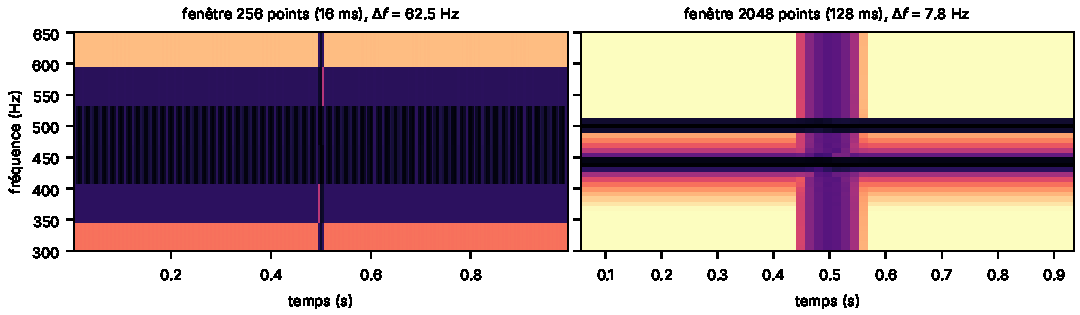
\includegraphics[width=\textwidth]{fig/fig_stft.pdf}
\caption{Deux sinus à 440 et 500\,Hz et un clic à 0,5\,s (foncé = énergie élevée). Fenêtre courte (à gauche) : le clic est net mais les deux sinus fusionnent en une bande. Fenêtre longue (à droite) : les sinus sont séparés mais le clic s'étale sur la durée de la fenêtre. Calcul personnel.}\label{fig:stft}
\end{figure}

\begin{projet}
Les artefacts de codecs sont des \emph{pics fins et stationnaires} (§\ref{sec:artefacts}) : ils demandent une \emph{longue} fenêtre ($\Delta f$ bien inférieur à l'espacement des pics) et se moyennent dans le temps sans perte. À l'inverse, un spectrogramme à courte fenêtre ou mel les efface. Ce choix de représentation est une \emph{ablation} du projet (§\ref{sec:detect}).
\end{projet}

\subsection{Représentations : amplitude, dB, mel, log-fréquence, CQT\nref{N3}}
\label{sec:repr}
Le spectrogramme est $|X[m,k]|$ (amplitude) ou $|X|^2$ (puissance) ; on le passe en décibels, $20\log_{10}|X|$, car l'oreille et la dynamique musicale sont logarithmiques. La phase est souvent jetée : le meilleur résultat d'Afchar et al. vient de l'\emph{amplitude} seule\sV. Trois façons de recadrer l'axe des fréquences :
\begin{itemize}
  \item \textbf{Mel} : $m=2595\log_{10}(1+f/700)$\sM, des filtres triangulaires étroits en grave et larges en aigu. Les MFCC sont la DCT du log-mel (timbre, parole). Les filtres larges moyennent \emph{plusieurs bins} : ils effacent les pics fins.
  \item \textbf{Log-fréquence} : un octave est un doublement ($A_2{=}110$, $A_3{=}220$, $A_4{=}440$\,Hz), un demi-ton un facteur $2^{1/12}$.
  \item \textbf{CQT} (\emph{constant-Q}) : $f_k=f_{\min}2^{k/B}$ avec $B$ bins par octave, largeur de bin $\propto f_k$, donc $Q=f_k/\delta f_k=1/(2^{1/B}-1)$ constant, et fenêtre de longueur $N_k\ensuremath{\approx}Qf_s/f_k$ : longue en grave, courte en aigu.
\end{itemize}
Intérêt pour un réseau : les harmoniques d'une note de fondamentale $f_0$ sont en $nf_0$ ; sur un axe \emph{linéaire}, leur espacement vaut $f_0$ (le motif change avec la hauteur) ; sur un axe \emph{logarithmique}, leurs positions sont $\log f_0+\log n$ : le motif est \emph{identique, simplement translaté} de $\log f_0$ (figure~\ref{fig:logaxis}). Un CNN, équivariant aux translations, en profite. Müller et al. trouvent que CQT et log-spectrogramme font environ 37\,\% d'EER de moins que le mel en moyenne, pour la détection de fausses voix\sV{} (leur jeu « in the wild » compte 37,9\,h et les EER se dégradent jusqu'à environ 1\,000\,\% hors du jeu d'entraînement ; des entrées de 4\,s font moins bien que des extraits entiers).

\begin{figure}[ht]
\centering
\begin{tikzpicture}[font=\scriptsize]
% (a) axe linéaire
\begin{scope}
\draw[->] (0,0)--(7.4,0) node[right]{Hz};
\foreach \n in {1,...,9}{\pgfmathsetmacro{\x}{7*\n*220/2000}\draw[red!70!black,line width=0.9pt] (\x,0)--(\x,0.75);}
\foreach \n in {1,...,6}{\pgfmathsetmacro{\x}{7*\n*330/2000}\draw[blue!70!black,line width=0.9pt] (\x,0)--(\x,0.45);}
\foreach \f in {0,500,1000,1500,2000}{\pgfmathsetmacro{\x}{7*\f/2000}\draw (\x,0.04)--(\x,-0.04) node[below]{\f};}
\node[anchor=north] at (3.5,-0.6) {(a) axe linéaire : espacements $220$ et $330$ Hz};
\end{scope}
% (b) axe log
\begin{scope}[xshift=9cm]
\draw[->] (0,0)--(7.4,0) node[right]{Hz};
\foreach \n in {1,...,9}{\pgfmathsetmacro{\x}{7*ln(\n*220/200)/ln(10)}\draw[red!70!black,line width=0.9pt] (\x,0)--(\x,0.75);}
\foreach \n in {1,...,6}{\pgfmathsetmacro{\x}{7*ln(\n*330/200)/ln(10)}\draw[blue!70!black,line width=0.9pt] (\x,0)--(\x,0.45);}
\foreach \f in {200,400,800,1600}{\pgfmathsetmacro{\x}{7*ln(\f/200)/ln(10)}\draw (\x,0.04)--(\x,-0.04) node[below]{\f};}
\draw[<->,thick,green!40!black] (0.29,0.95)--(1.52,0.95) node[midway,above]{$\log 1{,}5$};
\node[anchor=north] at (3.5,-0.6) {(b) axe log : même motif, translaté};
\end{scope}
\end{tikzpicture}
\caption{Harmoniques de deux notes ($f_0=220$\,Hz en rouge, $330$\,Hz en bleu, rapport $3/2$). En axe logarithmique, la seconde est la première translatée de $\log 1{,}5$ : c'est la propriété que M3 exploite pour la vitesse (§\ref{sec:robust}).}\label{fig:logaxis}
\end{figure}

\subsection{Rééchantillonnage, vitesse, hauteur, étirement\nref{N4}}\label{sec:resamp}
Quatre opérations qu'il faut ne \emph{jamais} confondre :
\begin{itemize}
  \item \textbf{Rééchantillonner} ($f_1\to f_2$) : le contenu en Hz ne bouge pas ; on suréchantillonne (insertion de zéros, puis filtre) et/ou on décime (filtre anti-repliement, puis sous-échantillonnage). Passer à 16\,kHz coupe tout au-dessus de 8\,kHz.
  \item \textbf{Changer la vitesse} d'un facteur $a$ : lire les mêmes échantillons à un autre rythme. Toutes les fréquences sont multipliées par $a$, la durée est divisée par $a$ : $f'=af$, soit $\log f'=\log f+\log a$ (une \emph{translation} en log-fréquence, de $12\log_2 a$ demi-tons : $\times0{,}7\to-6{,}2$, $\times1{,}1\to+1{,}7$, $\times1{,}4\to+5{,}8$).
  \item \textbf{Étirer} le temps : changer la durée sans toucher à la hauteur (vocodeur de phase) ; le spectre reste en place en Hz.
  \item \textbf{Décaler la hauteur} (\emph{pitch shift}) : étirement puis changement de vitesse pour retrouver la durée d'origine.
\end{itemize}
Effet sur un « peigne » de pics $nf_0$ (§\ref{sec:artefacts}) : un rééchantillonnage ne le déplace pas ; un étirement non plus ; un changement de vitesse ou de hauteur le remplace par $nf_0'$ avec $f_0'=af_0$, ce qui casse un détecteur calé en Hz mais est une pure translation sur l'axe log. Cela cadre avec les observations d'Afchar et al. (stable sous étirement, fragile sous décalage de hauteur)\sV, \emph{interprétation} de ma part.

\subsection{Compression MP3 et ingénierie audio pratique\nref{N5, N27}}\label{sec:mp3}
Le MP3 est un codage \emph{avec perte} fondé sur la perception : un modèle psychoacoustique estime quels sons sont masqués par leurs voisins (25 bandes critiques ; masquage temporel de 50 à 200\,ms), une transformée en cosinus discrète modifiée (MDCT) découpe le signal en lignes spectrales, on quantifie grossièrement ce qui est masqué, puis on code sans perte (Huffman). Un CD à 1\,411\,kbit/s passe à 128\,kbit/s, soit environ 11:1\sR. Détails de bas niveau (banc de 32 sous-bandes, 576 lignes spectrales par granule)\sM.

Ce qui compte pour le projet est la \textbf{coupure passe-bas} : l'encodeur supprime les hautes fréquences à bas débit, et FMA entier est en MP3. J'ai \emph{mesuré} cette coupure (ffmpeg~6.1.1, libmp3lame, bruit blanc stéréo à 44,1\,kHz, fréquence où le spectre moyen passe 30\,dB sous son niveau médian) :

\begin{center}\small
\begin{tabular}{@{}lrrrrrr@{}}
\toprule
Débit (kbit/s) & 64 & 96 & 128 & 192 & 256 & 320\\
Coupure mesurée (kHz) & 11,0 & 15,2 & 16,7 & 18,8 & 19,5 & 20,2\\
\bottomrule
\end{tabular}
\end{center}
\begin{figure}[ht]
\centering
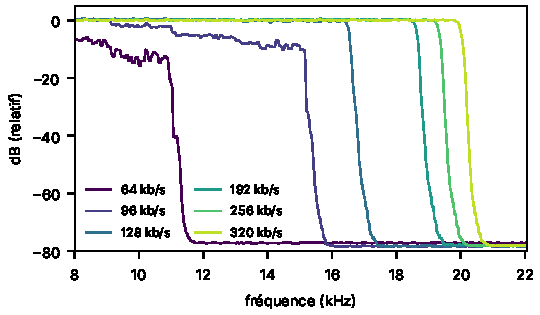
\includegraphics[width=0.62\textwidth]{fig/fig_mp3.pdf}
\caption{Spectre moyen d'un bruit blanc stéréo à 44,1\,kHz après passage MP3 (ffmpeg~6.1.1, libmp3lame), aux six débits du tableau. Mesure personnelle (lab L2).}\label{fig:mp3}
\end{figure}
En mono, la même mesure à 128\,kbit/s donne environ 20\,kHz : la coupure dépend du mode, du débit \emph{et} de l'encodeur (mesurer, ne pas supposer ; lab L2). Sur un signal musical réel d'autres effets s'ajoutent. Enfin, ffmpeg compense le retard de l'encodeur grâce à l'en-tête du fichier (mesuré : 0 échantillon de décalage) ; ce n'est pas vrai de tous les décodeurs.

\textbf{Ingénierie.} Quelques commandes suffisent à construire la chaîne du §\ref{sec:chaine} :
\begin{lstlisting}[language=bash]
ffmpeg -i in.mp3 -ac 1 -ar 16000 -af aresample=resampler=soxr out.wav   # mono, 16 kHz
ffmpeg -i in.wav -c:a libmp3lame -b:a 128k attaque.mp3                  # attaque MP3
ffmpeg -i in.wav -af loudnorm=I=-23 norm.wav                            # normalisation LUFS (EBU R128)
\end{lstlisting}
Niveau : RMS en dBFS $=20\log_{10}\sqrt{\overline{x^2}}$ (la sonie en LUFS pondère les fréquences). Toujours conserver le même filtre de rééchantillonnage pour les deux classes.

% ==================================================================
\section{Chaîne commune, raccourcis et contrôles négatifs}\label{sec:chaine}
% ==================================================================

\subsection{Le raccourci : définition et précédents\nref{N19}}
Geirhos et al. (arXiv 2004.07780)\sV{} appellent \emph{shortcut learning} le cas où un modèle résout une tâche par une règle de décision qui réussit sur le test i.i.d. mais échoue dès que les conditions changent (test hors distribution). Ils distinguent, parmi toutes les règles possibles, celles qui réussissent à l'entraînement, puis celles qui réussissent en i.i.d. (dont les \emph{raccourcis}), enfin la \emph{solution voulue}, qui généralise aussi hors distribution. Exemples : une vache reconnue par l'herbe, un classifieur de pneumonie qui lit la marque de l'hôpital, BERT qui détecte le mot « not ». Trois origines : les \emph{données} (biais systématiques), la \emph{règle de décision} (l'apprentissage discriminatif retient n'importe quel indice suffisant) et le \emph{biais inductif}. Trois conseils de diagnostic : n'attribuer une capacité de haut niveau que si aucun raccourci ne l'explique (« canon de Morgan »), comparer à des baselines fortes qui \emph{n'ont pas accès} à la caractéristique voulue, remplacer les tests i.i.d. par des tests hors distribution.

Trois précédents audio, directement transposables :
\begin{itemize}
  \item \textbf{Silence} (Müller et al., arXiv 2106.12914)\sV{} : dans ASVspoof~2019, les enregistrements authentiques ont des silences initiaux et finaux plus longs. Un réseau dense qui ne voit \emph{que} la durée du silence initial atteint un EER de 15,12\,\% (hasard : 50\,\%) ; rogner le silence fait passer RawNet2 de 3,61\,\% à 15,50\,\% d'EER ; ajouter la durée du silence comme caractéristique n'aide pas (les modèles l'extraient déjà). Leçon des auteurs, que je retiens : le silence n'est pas illégitime en soi, c'est sa répartition inégale qui l'est ; il faut l'équilibrer ou le supprimer.
  \item \textbf{Format} (Oh, ArtifactNet)\sV{} : avant un entraînement conscient des codecs, le modèle classait comme IA 98,7\,\% des pistes FMA en MP3 ; après, 8,0\,\% sur un sous-ensemble de 1\,350 pistes MP3 « difficiles ».
  \item \textbf{Généralisation} (Müller et al. 2022)\sV{} : hors du jeu d'entraînement, les EER se dégradent jusqu'à environ 1\,000\,\%.
\end{itemize}

\subsection{Inventaire des raccourcis possibles ici}
\begin{center}\footnotesize
\begin{tabularx}{\textwidth}{@{}L{2.9cm}XL{4.6cm}@{}}
\toprule
\textbf{Indice} & \textbf{Pourquoi il fuit} & \textbf{Neutralisation / mesure}\\
\midrule
Bande passante, fréquence native & FMA est en MP3 (coupure passe-bas) ; les générateurs ont des fréquences natives différentes (16, 32, 44,1\,kHz) & Rééchantillonnage commun ; caractéristique « bande passante » dans M0\\
Format et codec amont & MP3 contre WAV ; l'artefact d'un MP3 se confond avec celui d'un codec & Même chaîne pour les deux classes ; M0 ; attaque MP3 \emph{explicite}\\
Durée, silences, début/fin & Génération par fenêtres de 10\,s ; silences de début de piste & Segments de 10\,s à position aléatoire ; silence dans M0 ; modèle « silence seul »\\
Niveau sonore & Normalisation différente selon la source ; écrêtage & Normalisation commune (RMS ou LUFS) ; niveau dans M0\\
Mono/stéréo, bits, étiquettes (ID3) & Métadonnées de fichier & Tout convertir (mono, 16\,kHz, flottant) ; jeter les étiquettes\\
Contenu (artiste, genre, voix) & Deux extraits d'un même artiste se ressemblent & Découpage \emph{par artiste} (et par légende pour les générateurs)\\
\bottomrule
\end{tabularx}
\end{center}

\subsection{La chaîne commune}
Principe (figure~\ref{fig:projet}) : les deux classes subissent \emph{exactement les mêmes} opérations, sauf celle que l'on veut détecter. Pour un morceau FMA $x$ et un codec de fréquence native $f_c$ (24\,kHz pour EnCodec, 44,1\,kHz pour DAC) :
\[
\text{réel : } x\xrightarrow{\ \text{mono}\ }\xrightarrow{\ \to f_c\ }\xrightarrow{\ \to16\,\text{kHz}\ }\ \text{niveau}\to\text{segments}\qquad
\text{faux : } x\xrightarrow{\ \text{mono}\ }\xrightarrow{\ \to f_c\ }\boxed{\text{codec}}\xrightarrow{\ \to16\,\text{kHz}\ }\ \text{niveau}\to\text{segments}
\]
avec le même rééchantillonneur (\texttt{soxr}), le même niveau cible et les mêmes segments de 10\,s. Conséquences à connaître : (i) le MP3 d'origine est présent dans les deux classes, il ne discrimine pas ; (ii) la fréquence d'ancrage de 16\,kHz borne l'analyse à 8\,kHz, donc, pour EnCodec 24\,kHz (un pic tous les 75\,Hz, §\ref{sec:artefacts}), à environ 106 pics au lieu de 160 ; (iii) on ne peut rien conclure sur les artefacts au-dessus de 8\,kHz (les papiers de Deezer travaillent en 5--16\,kHz\sV).

\subsection{Détecteur de métadonnées M0 et contrôles\nref{N20}}
\textbf{M0} est un classifieur qui ne voit \emph{aucun signal audio}, seulement des descripteurs du fichier : durée, fréquence native, bande passante estimée (plus haute fréquence dont le niveau dépasse $-60$\,dB), niveau RMS, proportion d'échantillons nuls, durée de silence initial, écrêtage. On entraîne (régression logistique ou arbres) sur les mêmes découpages et l'on rapporte l'AUC avec un intervalle de confiance bootstrap groupé (§\ref{sec:incertitude}). \hyp{si la chaîne est saine, M0 est au hasard} ; un intervalle qui exclut 0,5 prouve un raccourci, qu'il faut corriger \emph{avant} d'interpréter les autres détecteurs (précisément la démarche de Müller et al.). On parle de \emph{M0 résiduel} quand on le mesure \emph{après} la chaîne commune.

Contrôles à prévoir :
\begin{itemize}
  \item \textbf{négatifs} (doivent donner AUC $\ensuremath{\approx}0{,}5$) : M0 ; étiquettes permutées ; modèle « silence seul » ;
  \item \textbf{positif} (doit donner AUC $\ensuremath{\approx}1$) : un détecteur entraîné \emph{et testé} sur le même codec, preuve que l'instrument voit l'artefact quand il existe.
\end{itemize}
Une expérience sans contrôle ne prouve rien : si le positif échoue, le montage est défaillant ; si le négatif dépasse 0,5, il y a une fuite.

% ==================================================================
\section{Apprentissage et évaluation}\label{sec:eval}
% ==================================================================

\subsection{CNN sur spectrogramme\nref{N6}}
Un spectrogramme se traite comme une image (fréquence $\times$ temps), mais \emph{les deux axes ne sont pas équivalents} (slides de G.~Richard, MVA\sV) : décaler un événement dans le temps le laisse inchangé, alors que décaler un spectre de $\Delta f$ sur un axe \emph{linéaire} ne revient pas à changer la hauteur (les harmoniques s'espacent autrement, §\ref{sec:repr}). Sur un axe logarithmique, si. Trois notions suffisent :
\begin{itemize}
  \item \textbf{Convolution et équivariance} : un filtre appris glisse sur l'image ; translater l'entrée translate la carte de sortie.
  \item \textbf{Pooling} : le max-pooling rend la sortie (approximativement) \emph{invariante} à de petits décalages, au prix de la résolution. Pour un détecteur de pics fins, pooler trop tôt l'axe des fréquences peut détruire l'indice : à ablater.
  \item \textbf{Champ réceptif} : avec $r_0=1$, $j_0=1$ (saut), une couche de noyau $k$ et de pas $s$ donne $r_l=r_{l-1}+(k-1)\,j_{l-1}$ et $j_l=j_{l-1}\,s$. Trois convolutions $3\times3$ sans pas : $r=7$. Avec un max-pooling $2\times2$ (pas~2) après chaque convolution : $r=3\to4\to8\to10\to18\to22$ ; on voit $22\times22$ pixels.
\end{itemize}
Les convolutions dilatées et les pas élargissent le champ sans multiplier les paramètres (MVA, \S7). Le CNN d'Afchar et al.\sV{} a six couches convolutives, environ 1,6\,M de paramètres, et lit un spectrogramme d'amplitude sur des extraits de 0,8\,s. Pour le choix des entrées et des couches, le tutoriel de Choi et al. (arXiv 1709.04396)\sV{} fait référence (représentations d'entrée, convolutions 1D et 2D, pooling, conseils de conception) ; il ne traite \emph{pas} des fuites entre artistes (§\ref{sec:incertitude}).

\subsection{Transformers sur spectrogramme\nref{N7}}
L'\emph{Audio Spectrogram Transformer} (AST, arXiv 2104.01778)\sR{} découpe le spectrogramme en patchs, les projette en jetons et applique de l'attention : c'est le premier classifieur audio sans convolution (AudioSet 0,485\,mAP, ESC-50 95,6\,\%, Speech Commands~V2 98,1\,\%)\sR ; log-mel à 128 bandes, patchs $16\times16$ avec recouvrement et initialisation depuis un ViT/DeiT d'ImageNet\sM. Le nombre de jetons d'un découpage en patchs 2D croît comme le \emph{produit} (temps)$\times$(fréquence). \textbf{SpecTTTra} (SONICS, arXiv 2408.14080)\sV{} tokenise séparément le temps et la fréquence par des convolutions 1D : la croissance devient \emph{additive}, ce qui permet des extraits longs (F1 de 0,97 à 120\,s ; au contraire, à 5\,s c'est ConvNeXt qui est le meilleur, 0,90). Le projet n'utilise SpecTTTra qu'en \emph{inférence} (M4, point de comparaison externe).

\subsection{Métriques de détection et calibration\nref{N8}}
Un détecteur produit un score $s(x)$ (« faux » si $s>\tau$). Les taux de vrais et de faux positifs sont $\TPR(\tau)=P(s>\tau\mid y{=}1)$ et $\FPR(\tau)=P(s>\tau\mid y{=}0)$ ; la courbe ROC les trace en balayant $\tau$.
\begin{itemize}
  \item \textbf{AUC} : aire sous la ROC, égale à $P\big(s(X^+)>s(X^-)\big)$ (plus $\tfrac12$ pour les égalités) : la probabilité qu'un faux tiré au hasard ait un score supérieur à celui d'un réel, soit $\AUC=\frac1{n^+n^-}\sum_{i}\sum_{j}\mathbf 1[s_i^+>s_j^-]$ (statistique de Mann--Whitney). $\AUC=0{,}5$ signifie « hasard ». Elle ne dépend que du \emph{rang} des scores.
  \item \textbf{EER} : valeur commune de $\FPR$ et de $1-\TPR$ ; \textbf{$\tprfpr$} : taux de détection quand on tolère 1\,\% de faux positifs (point de fonctionnement réaliste).
\end{itemize}
\emph{Exemple à six scores} : faux $\{0{,}9;\,0{,}8;\,0{,}4\}$, réels $\{0{,}7;\,0{,}3;\,0{,}2\}$. Sur les 9 paires (faux, réel), 8 sont bien ordonnées (seule $0{,}4<0{,}7$ échoue) : $\AUC=8/9\ensuremath{\approx}0{,}89$. Pour $\tau=0{,}5$ : $\TPR=2/3$, $\FPR=1/3$, donc $\EER=1/3$ (vérifié avec scikit-learn).

\textbf{Pourquoi l'AUC ne suffit pas.} Elle est invariante à toute transformation monotone des scores, mais l'exactitude et le F1 dépendent du seuil $\tau$ figé sur le jeu d'entraînement. Si la distribution des scores se décale (autre générateur, attaque), l'AUC peut rester haute et le F1 s'effondrer : Dugelay et al. rapportent, sous décalage de hauteur, AUC 0,963 mais F1 0,279\sV ; Park et al. insistent pour évaluer aussi le point de fonctionnement\sV. On rapporte donc l'AUC \emph{et} $\tprfpr$ avec un seuil figé sur des données propres.

\textbf{Calibration} (Guo et al., arXiv 1706.04599)\sV. Un classifieur est calibré si $P(\hat Y=Y\mid\hat P=p)=p$. On la mesure par le \emph{diagramme de fiabilité} (exactitude par intervalle de confiance) et par l'\emph{ECE} : $\mathrm{ECE}=\sum_{m=1}^{M}\frac{|B_m|}{n}\,\big|\mathrm{acc}(B_m)-\mathrm{conf}(B_m)\big|$ ($M$ intervalles ; MCE : le maximum au lieu de la somme) ; on suit aussi la NLL. Le \emph{temperature scaling} divise les logits par un scalaire $T>0$ ajusté en minimisant la NLL sur un jeu de validation : il ne change ni l'argmax ni l'ordre des scores, donc ni l'exactitude ni l'AUC. Les auteurs notent que la normalisation par lots, une faible régularisation et une grande capacité dégradent la calibration. Le score de Brier $\overline{(p-y)^2}$ est un complément usuel\sM. Afchar et al. observent des sorties presque toujours proches de 0 ou 1, avec la classe « réel » comme défaut sous perturbation\sV : la calibration y est un vrai sujet.
\begin{figure}[ht]
\centering
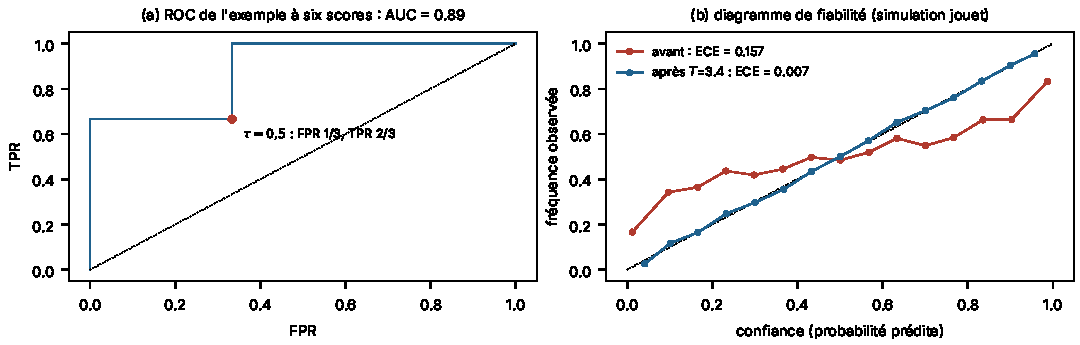
\includegraphics[width=\textwidth]{fig/fig_roc_calib.pdf}
\caption{(a)~ROC de l'exemple à six scores ($\AUC=8/9$). (b)~Simulation jouet de 20\,000 exemples à logits sur-confiants : le \emph{temperature scaling} ($T=3{,}4$, par minimisation de la NLL ; ajusté ici sur les mêmes données par simplicité, en pratique sur une validation) ramène l'ECE de 0,157 à 0,007 sans toucher à l'AUC (0,827 avant et après). Calculs personnels.}\label{fig:roc}
\end{figure}

\subsection{Incertitude, comparaisons, découpages\nref{N9, N26}}\label{sec:incertitude}
\textbf{Découper par groupe.} Deux extraits d'un même morceau, ou de deux morceaux d'un même artiste, partagent timbre, mastering, voix : un découpage aléatoire laisse fuiter l'information entre entraînement et test et gonfle les scores. On découpe donc \emph{par artiste} pour FMA (identifiant d'artiste dans \texttt{tracks.csv}) et \emph{par légende} pour FakeMusicCaps (une légende produit un extrait par générateur). Chaque extrait de 10\,s est une \emph{unité corrélée} à ses voisins.

\textbf{Bootstrap groupé.} Pour un intervalle de confiance sur l'AUC, on tire les \emph{groupes} (artistes, légendes) avec remise, on recalcule l'AUC, on répète ($B=1\,000$ à $10\,000$) et l'on prend les centiles 2,5\,\% et 97,5\,\%. Tirer les extraits individuellement sous-estimerait l'incertitude. \textbf{Test apparié} : pour comparer deux détecteurs A et B, on tire les \emph{mêmes} groupes pour les deux et l'on calcule $\Delta\AUC=\AUC_A-\AUC_B$ ; un intervalle qui exclut 0 est la convention « A fait mieux » du projet (alternative : le test de DeLong). Avec $m$ comparaisons, la \emph{correction de Holm} classe les $p$-valeurs $p_{(1)}\le\dots\le p_{(m)}$ et rejette $H_{(i)}$ tant que $p_{(i)}\le\alpha/(m-i+1)$.
\begin{lstlisting}[language=Python]
def boot_delta(y, sA, sB, g, B=2000, seed=0):             # y: etiquettes, sA/sB: scores, g: groupe
    rng = np.random.default_rng(seed); G = np.unique(g)
    idx = {k: np.flatnonzero(g == k) for k in G}; d = []
    for _ in range(B):
        i = np.concatenate([idx[k] for k in rng.choice(G, len(G), replace=True)])
        if len(np.unique(y[i])) == 2:                      # memes groupes pour A et B
            d.append(roc_auc_score(y[i], sA[i]) - roc_auc_score(y[i], sB[i]))
    return np.percentile(d, [2.5, 97.5])
\end{lstlisting}
\textbf{Trois variabilités distinctes}, à ne pas confondre : le \emph{bootstrap} mesure la variabilité due au \emph{jeu de test fini} ; la \emph{variance entre graines} celle de l'\emph{entraînement} ; la \emph{variabilité des données} celle du choix du jeu d'entraînement. Aucune ne remplace les autres (lab L7).

\begin{projet}
Conventions du projet : « au-dessus du hasard » = l'IC à 95\,\% de l'AUC (bootstrap groupé) exclut 0,5 ; « mieux » = l'IC à 95\,\% apparié de $\Delta\AUC$ exclut 0 ; « transfert fort » = $\AUC\ge0{,}90$ (seuil indicatif, à valider avec l'encadrant).
\end{projet}

% ==================================================================
\section{Génération audio neuronale : d'où viennent les artefacts}\label{sec:gen}
% ==================================================================

\subsection{Auto-encodeurs, VAE, GAN, diffusion\nref{N10, N11, N16}}
Un \textbf{auto-encodeur} compresse $x$ en $z=E(x)$ puis le reconstruit, $\hat x=D(z)$, en minimisant $\|x-\hat x\|^2$ ; le goulot d'étranglement force à ne garder que l'essentiel. Un \textbf{VAE} fait produire à l'encodeur une moyenne $\mu$ et un écart-type $\sigma$, tire $z=\mu+\sigma\odot\varepsilon$ ($\varepsilon\sim\mathcal N(0,I)$, \emph{reparamétrisation}) et maximise la borne $\mathbb E_q[\log p(x\mid z)]-\mathrm{KL}\big(q(z\mid x)\,\|\,p(z)\big)$ (Weng, VAE\sV). Un \textbf{GAN} oppose un générateur $G$ à un discriminateur $D$ : $\min_G\max_D\ \mathbb E[\log D(x)]+\mathbb E[\log(1-D(G(z)))]$. Les codecs et les vocodeurs (HiFi-GAN) utilisent des variantes : perte \emph{hinge} ($L_D=\mathbb E[\max(0,1-D(x))]+\mathbb E[\max(0,1+D(\hat x))]$, $L_G=-\mathbb E[D(\hat x)]$, forme usuelle\sM) sur plusieurs discriminateurs (formes d'onde à plusieurs échelles, STFT), plus une perte de \emph{feature matching} (distance entre les activations du discriminateur sur $x$ et $\hat x$) et une perte spectrale multi-échelle sur mel. Les \textbf{modèles de diffusion} (Weng, diffusion\sV) bruitent $x_0$ par $q(x_t\mid x_{t-1})=\mathcal N(\sqrt{1-\beta_t}\,x_{t-1},\beta_t I)$, ce qui donne en forme close $x_t=\sqrt{\bar\alpha_t}\,x_0+\sqrt{1-\bar\alpha_t}\,\varepsilon$ avec $\bar\alpha_t=\prod_{s\le t}(1-\beta_s)$ ; un réseau $\varepsilon_\theta$ apprend à prédire le bruit, $L=\mathbb E\|\varepsilon-\varepsilon_\theta(x_t,t)\|^2$, puis on inverse le processus. La \emph{diffusion latente} fait cela dans l'espace $z$ d'un VAE, conditionnée par du texte via de l'attention croisée, avec le \emph{guidage sans classifieur} $\tilde\varepsilon=(w+1)\varepsilon_\theta(x_t,c)-w\,\varepsilon_\theta(x_t)$.

\textbf{Idée directrice} : quelle que soit la machinerie en amont (LM, diffusion, quantification), la \emph{dernière étape} --- décodeur de codec, décodeur de VAE, vocodeur --- transforme une représentation à basse cadence en forme d'onde par des couches de \emph{suréchantillonnage}. C'est là que naît l'empreinte.

\subsection{Suréchantillonnage et origine des pics spectraux\nref{N12, N25}}\label{sec:artefacts}
\textbf{Convolution transposée.} Avec un pas $s$ et un noyau de taille $K$, elle insère $s-1$ zéros entre les échantillons d'entrée, puis convolue avec le noyau appris : $y[n]=\sum_i x[i]\,h[n-si]$, de longueur $(L-1)s+K$. Si $K$ n'est pas multiple de $s$, le recouvrement est \emph{inégal} : avec $K=3$, $s=2$, les sorties reçoivent alternativement 2 et 1 contributions ; avec $K=5$, $s=3$, le motif est $1,2,2,1,2,2,\dots$ (vérifié par un petit calcul). Distill (Odena et al.)\sV{} montre que ces motifs en damier apparaissent même à l'initialisation aléatoire ; le remède est de redimensionner (plus proche voisin) \emph{puis} de convoluer. Pons et al. (arXiv 2010.14356)\sR{} distinguent des artefacts \emph{tonaux} (dus à l'insertion de zéros) et de \emph{filtrage}, et retiennent le plus proche voisin comme meilleur compromis ; les notebooks de Dolby (licence MIT)\sV{} permettent de les reproduire (conv. transposée, plus proche voisin, interpolation linéaire, sous-pixel).

\textbf{Explication de Fourier.} Le théorème de convolution donne $\mathcal F[s*r]=\mathcal F[s]\cdot\mathcal F[r]$. Insérer des zéros avec un facteur $k$ donne $u[n]=s[n/k]$ si $k\mid n$, sinon $0$, donc $U(e^{i\omega})=\sum_m s[m]e^{-i\omega km}=S(e^{ik\omega})$ : le spectre est comprimé d'un facteur $k$ et \emph{répliqué} $k$ fois (figure~\ref{fig:repliques}b) ; le filtre $r$ appris qui suit n'élimine ces images qu'imparfaitement. Afchar et al. (ISMIR 2025, arXiv 2506.19108)\sR{} en tirent que, si $f_{\mathrm e}$ est la cadence \emph{avant} suréchantillonnage, la sortie présente des pics aux fréquences $n f_{\mathrm e}$, $n\in\{0,\dots,\lfloor k/2\rfloor\}$ ; avec $L$ couches, $P_{\max}=\prod_i k_i$ et $\lfloor P_{\max}/2\rfloor+1$ pics. Pour EnCodec, les pas $\{8,5,4,2\}$ donnent $P_{\max}=320$ et \textbf{161 pics}, un tous les 75\,Hz jusqu'à 12\,kHz. Intuition temporelle : un motif qui se répète toutes les 320 échantillons (13,3\,ms à 24\,kHz) a pour spectre des raies aux multiples de $24\,000/320=75$\,Hz. Ils dépendent de l'\emph{architecture} (les pas), non des poids ni des données (vérifié sur DAC par plusieurs graines et jeux de données) ; leur \emph{amplitude}, elle, dépend des filtres.

\begin{figure}[ht]
\centering
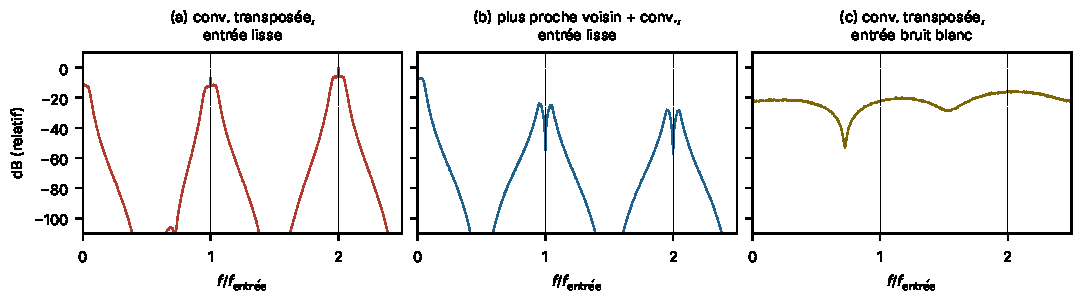
\includegraphics[width=\textwidth]{fig/fig_upsampling.pdf}
\caption{Spectre moyen (400 réalisations) d'un suréchantillonneur jouet : facteur~5, noyau~7, poids aléatoires. (a)~Conv. transposée, entrée \emph{lisse} (basses fréquences plus composante continue) : lobes à $0$, $f_{\mathrm e}$, $2f_{\mathrm e}$ d'amplitude comparable. (b)~Plus proche voisin puis conv. : lobes en $f_{\mathrm e}$ et $2f_{\mathrm e}$ creusés, environ 20\,dB plus bas dans ce tirage. (c)~Conv. transposée, entrée en \emph{bruit blanc} : spectre moyen lisse, sans pics. Mesure personnelle (lab L4).}\label{fig:upsampling}
\end{figure}

La figure~\ref{fig:upsampling}c corrige un piège : avec un bruit blanc en entrée, la périodicité du suréchantillonnage se voit dans la \emph{variance temporelle} (période $s$) mais pas dans le spectre de puissance moyen. Les pics exigent une entrée \emph{structurée en basses fréquences}, comme les représentations latentes lisses d'un codec ou une composante continue (biais).

\begin{center}\footnotesize
\begin{tabularx}{\textwidth}{@{}L{4.6cm}rrrX@{}}
\toprule
\textbf{Décodeur} & $f_{\mathrm e}$ & $P_{\max}$ & \textbf{Pics} & \textbf{Remarque}\\
\midrule
EnCodec 24\,kHz (strides $8,5,4,2$) & 75\,Hz & 320 & 161 & jusqu'à 12\,kHz\\
EnCodec 32\,kHz (MusicGen) & 50\,Hz & 640 & 321 & jusqu'à 16\,kHz\\
DAC 44,1\,kHz (86\,Hz) & 86\,Hz & $\ensuremath{\approx}512$ & $\ensuremath{\approx}257$ & jusqu'à 22\,kHz\\
VAE de Stable Audio Open (21,5\,Hz) & 21,5\,Hz & $\ensuremath{\approx}2\,048$ & $\ensuremath{\approx}1\,025$ & un pic tous les 21,5\,Hz\\
\bottomrule
\end{tabularx}
\end{center}
\emph{Calculs personnels} d'après les cadences annoncées ($P_{\max}=f_{\mathrm{audio}}/f_{\mathrm e}$), valables si tout le suréchantillonnage se fait par insertion de zéros ; un décodeur à plus proche voisin ou à Snake se comporte autrement. À 16\,kHz (ancrage du projet), il ne reste que les pics sous 8\,kHz.

\subsection{Quantification vectorielle et codecs neuronaux\nref{N13, N14}}\label{sec:codecs}
\textbf{VQ.} Un dictionnaire (\emph{codebook}) de $K$ vecteurs $c_j$ remplace $z$ par son plus proche voisin, $q(z)=c_{j^\star}$, $j^\star=\arg\min_j\|z-c_j\|$ ; on l'entraîne (VQ-VAE) par \emph{straight-through} (copie du gradient) avec $L=\|x-D(e)\|^2+\|\mathrm{sg}[z_e]-e\|^2+\beta\|z_e-\mathrm{sg}[e]\|^2$ (reconstruction, dictionnaire, engagement ; $\mathrm{sg}$ : arrêt de gradient), ou par moyenne mobile exponentielle du dictionnaire (Weng\sV). \textbf{RVQ} : plusieurs quantificateurs en cascade, chacun quantifiant le \emph{résidu} du précédent : $r_0=z$, $k_q=\arg\min_j\|r_{q-1}-c^q_j\|$, $r_q=r_{q-1}-c^q_{k_q}$, $\hat z=\sum_q c^q_{k_q}$ (AssemblyAI\sV). Le débit est $R=f_{\mathrm{trame}}\times N_q\times\log_2K$ : plus de codebooks, plus de débit, meilleure reconstruction.

\begin{figure}[ht]
\centering
\begin{tikzpicture}[font=\scriptsize,box/.style={draw,rounded corners=2pt,align=center,inner sep=3pt,minimum height=0.85cm},arr/.style={-{Stealth[length=4pt]},line width=0.5pt}]
\node[box,fill=blue!6] (x) at (0,0) {$x$\\{[24\,kHz]}};
\node[box,fill=blue!6] (E) at (2.5,0) {Encodeur\\conv., pas $2,4,5,8$};
\node[box,fill=orange!15] (Q) at (5.6,0) {RVQ\\$N_q$ codebooks\\$K{=}1024$};
\node[box,fill=blue!6] (D) at (8.5,0) {Décodeur\\conv. transposées\\\textbf{suréchantillonnage}};
\node[box,fill=blue!6] (xh) at (11.2,0) {$\hat x$};
\node[box,dashed,fill=green!8] (Dis) at (8.5,-1.6) {discriminateurs\\(STFT, multi-échelle)};
\draw[arr] (x)--(E); \draw[arr] (E)--node[above]{75\,Hz}(Q); \draw[arr] (Q)--node[above]{$\hat z$}(D); \draw[arr] (D)--(xh);
\draw[arr,dashed] (xh) |- (Dis.east);
\node[font=\scriptsize] at ([yshift=-0.35cm,xshift=-0.2cm]Q.south west) {$R=75\times N_q\times10$ bit/s};
\end{tikzpicture}
\caption{Codec neuronal de type EnCodec. $N_q=8$ donne $75\times8\times10=6$\,kbit/s. L'artefact vient du décodeur (zone grasse), pas de la quantification.}\label{fig:codec}
\end{figure}

\begin{center}\footnotesize
\begin{tabularx}{\textwidth}{@{}L{2.2cm}L{1.5cm}L{1.5cm}L{2.2cm}L{1.9cm}X@{}}
\toprule
\textbf{Codec} & $f_s$ & \textbf{Trames} & $N_q\times K$ & \textbf{Débit} & \textbf{Particularités}\\
\midrule
SoundStream\sV & 24\,kHz & 75\,Hz & 8$\times$1024 (ex.) & 3--18\,kbit/s & RVQ ; \emph{quantizer dropout} (nb. de codebooks tiré au hasard) ; discr. STFT + 3 formes d'onde ; $\lambda_{\mathrm{adv}}{=}1$, $\lambda_{\mathrm{feat}}{=}100$, $\lambda_{\mathrm{rec}}{=}1$\\
EnCodec\sV & 24 (mono), 48\,kHz (stéréo) & 75 / 150\,Hz & jusqu'à 32$\times$1024 & 1,5--24 ; 6--24\,kbit/s & LSTM ; reconstruction L1 + mel multi-échelle ; MS-STFT adversarial (hinge) + feature matching ; \emph{loss balancer} ; LM optionnel ($-40$\,\%)\\
DAC\sV & 44,1\,kHz (aussi 24, 16) & 86\,Hz & 9$\times$1024 & $\ensuremath{\approx}8$\,kbit/s ($\ensuremath{\approx}90\times$) & activation \emph{Snake} ; codebooks de 8 dim. normalisés $L_2$ ; dropout $p=0{,}5$ ; discr. STFT complexe multi-échelle et multi-bande\\
EnCodec de MusicGen\sV & 32\,kHz mono & 50\,Hz & 4$\times$2048 & $\ensuremath{\approx}2{,}2$\,kbit/s & jetons pour un modèle de langage\\
Mimi\sV & 24\,kHz & 12,5\,Hz & 8$\times$2048 & $\ensuremath{\approx}1{,}1$\,kbit/s & \emph{split RVQ} : 1 niveau sémantique (distillation WavLM) + 7 acoustiques ; Transformers causaux ; données d'entraînement non confirmées\\
\bottomrule
\end{tabularx}
\end{center}
Codec-SUPERB (arXiv 2402.13071)\sV{} compare 6 codecs (19 modèles) sur 20 jeux de données : DAC offre le meilleur compromis débit/qualité, AcademiCodec reste bon à 2--3\,kbit/s, EnCodec est une référence solide. \textbf{Musika} (arXiv 2208.08706)\sV{} n'est pas un RVQ : deux auto-encodeurs convolutifs empilés sur le spectrogramme STFT (magnitude et phase, iSTFT), un GAN générant dans l'espace latent, 22,05\,kHz.

\begin{projet}
\textbf{Un codec n'est pas un générateur} : il reçoit de la vraie musique et la « reconstruit » avec les défauts de son décodeur. Les faux de substitution du projet sont donc de la musique réelle \emph{vue à travers un décodeur}. \hyp{H1 : les artefacts viennent du décodeur ; un détecteur transfère mieux vers un générateur dont le décodeur ressemble à celui qui a fabriqué ses faux}. Dans la matrice détecteur $\times$ générateur, EnCodec (MusicGen) est le cas favorable.
\end{projet}

\subsection{Modèles de musique et fiche des cinq générateurs\nref{N15, N16}}
\textbf{MusicGen} (arXiv 2306.05284)\sV{} est un modèle de langage Transformer \emph{autorégressif} sur les jetons EnCodec (32\,kHz, 4 codebooks, 50\,Hz). Plutôt que d'aplatir les 4 flux (séquence $4\times$ plus longue), un \emph{motif d'entrelacement à retard} décale le codebook $k$ de $k{-}1$ pas : un seul passage prédit les 4 niveaux en parallèle. Tailles 300\,M, 1,5\,Md et 3,3\,Md de paramètres, environ 20\,000\,h de musique, conditionnement texte (T5) et mélodie (chroma). Les quatre autres générateurs de FakeMusicCaps sont à \textbf{diffusion latente} (§5.1) ; leur décodeur final est un VAE, parfois suivi d'un vocodeur.

\begin{center}\footnotesize
\begin{tabularx}{\textwidth}{@{}L{2.1cm}L{4.6cm}L{3.5cm}L{1.9cm}X@{}}
\toprule
\textbf{Générateur} & \textbf{Architecture} & \textbf{Décodeur final} & \textbf{Natif} & \textbf{Données}\\
\midrule
MusicGen (medium)\sV & LM sur jetons EnCodec ; T5 & décodeur EnCodec & 32\,kHz mono & $\ensuremath{\approx}20$\,k h\\
MusicLDM\sV & CLAP + diffusion latente (UNet) ; mel à 128 bandes ; mélange synchronisé sur le rythme & VAE + HiFi-GAN réentraîné sur la musique & 16\,kHz, 10,24\,s & ---\\
AudioLDM\,2 (musique)\sV & AudioMAE + GPT-2 + diffusion latente & VAE + HiFi-GAN (variante non précisée) & 16\,kHz & dont FMA (106\,574 pistes) et un sous-ensemble de MSD\\
Stable Audio Open\sV & VAE ($\ensuremath{\approx}156$\,M, Snake, 64 canaux latents, 21,5\,Hz) + DiT ($\ensuremath{\approx}1$\,Md) ; T5 & décodeur du VAE (sans tanh) & 44,1\,kHz stéréo & 486\,492 enregistrements ($\ensuremath{\approx}7\,300$\,h), Freesound + FMA (licences CC)\\
Mustango\sV & diffusion latente de type Tango, VAE d'AudioLDM, FLAN-T5, MuNet (rythme, accords) & non précisé dans la page lue & 16\,kHz, 10\,s max. & ---\\
\bottomrule
\end{tabularx}
\end{center}
FakeMusicCaps fournit tout en \textbf{mono 16\,kHz} : MusicGen et Stable Audio Open sont donc \emph{rééchantillonnés et mélangés en mono} par les auteurs du jeu, ce qui retire ce qui est au-dessus de 8\,kHz. Deux observations pour l'interprétation : les données d'entraînement de Stable Audio Open et d'AudioLDM\,2 contiennent FMA, c'est-à-dire potentiellement les « réels » du détecteur ; et le \textbf{décodeur oracle} du projet (passer de la vraie musique par l'encodeur--décodeur d'un générateur ouvert, sans la diffusion) fabrique des faux au plus près de ce générateur.

% ==================================================================
\section{Les détecteurs M0 à M4}\label{sec:detect}
% ==================================================================

\begin{center}\footnotesize
\begin{tabularx}{\textwidth}{@{}L{1.0cm}L{4.2cm}L{3.6cm}X@{}}
\toprule
 & \textbf{Entrée et modèle} & \textbf{Famille} & \textbf{Ce qu'il teste dans le projet}\\
\midrule
M0 & descripteurs de fichier ; régression logistique ou arbres & contrôle négatif & raccourcis (H3)\\
M1 & empreinte spectrale moyenne ; régression logistique ($\ensuremath{\approx}10^4$ paramètres) & artefact explicite & explication de Fourier (H1)\\
M2 & spectrogramme d'amplitude ; petit CNN ($\ensuremath{\approx}1{,}6$\,M de paramètres, à la Afchar) & appris & transfert hors famille (H1, H2)\\
M3 & spectre moyen en log-fréquence ; corrélation croisée, max-pooling & invariant à l'échelle & vitesse, hauteur, MP3 (H4)\\
M4 & SpecTTTra de SONICS, en inférence & référence externe & point de comparaison\\
\bottomrule
\end{tabularx}
\end{center}

\subsection{Empreintes spectrales (\emph{fakeprints}) : M1\nref{N17}}
Recette de Afchar et al. (arXiv 2506.19108)\sR{} : (1)~calculer l'amplitude de la STFT sur de nombreux segments et la \textbf{moyenner dans le temps}, ce qui fait ressortir les pics stationnaires et écrase la musique ; (2)~\textbf{soustraire} un minimum glissant (enveloppe inférieure locale) pour retirer la forme lente du spectre ; (3)~\textbf{restreindre} à une bande (5--16\,kHz dans l'article ; 1--8\,kHz pour SONICS à 16\,kHz) ; (4)~entraîner une \textbf{régression logistique linéaire} (environ $10^4$ paramètres : un poids par bin). Résultats annoncés : environ 99,7 à 100\,\% sur DAC, EnCodec et Musika ; Suno~v2/v3/v3.5 et Udio~130 $\ensuremath{\approx}$ 100\,\% ; mais Udio~32, non vu à l'entraînement, seulement 39,8\,\%. Limites reconnues : réseaux séquentiels simples étudiés, interpolation non entièrement démontrée, robustesse au rééchantillonnage et à la hauteur non testée.
\begin{lstlisting}[language=Python]
def fakeprint(x, sr=16000, n_fft=4096, band=(1000, 8000), w=101):    # schema pedagogique
    f, _, Z = sg.stft(x, sr, nperseg=n_fft, noverlap=n_fft // 2)
    m = np.log(np.abs(Z).mean(axis=1) + 1e-9)             # 1. spectre moyen (log)
    m = m - nd.minimum_filter1d(m, size=w)                # 2. retire l'enveloppe lente
    return m[(f >= band[0]) & (f <= band[1])]             # 3. bande ; 4. -> LogisticRegression
\end{lstlisting}
\begin{figure}[ht]
\centering
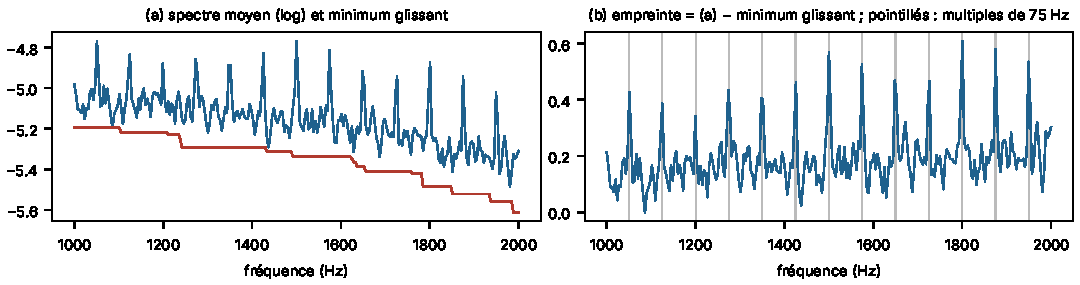
\includegraphics[width=\textwidth]{fig/fig_fakeprint.pdf}
\caption{Le croquis ci-dessus sur un signal synthétique (10\,s à 16\,kHz : bruit coloré plus un peigne à 75\,Hz). (a)~Le spectre moyen a une pente et un plancher ; le minimum glissant (rouge) suit le plancher. (b)~Une fois la pente retirée, les pics tombent sur les multiples de 75\,Hz. Calcul personnel.}\label{fig:fakeprint}
\end{figure}
Ce croquis est le mien, \emph{pas} le code de Deezer ; vérifié sur un bruit auquel on ajoute un peigne à 75\,Hz (les pics ressortent, niveau 0,39 contre 0,17 entre les pics ; sans peigne, 0,17 et 0,18). Le dépôt \texttt{deezer/ismir25-ai-music-detector} fournit \texttt{compute\_fakeprints.py}, \texttt{train\_test\_regressor.py} et un notebook de visualisation des latents EnCodec ; il demande FMA (avec le découpage du détecteur) et SONICS, est sous CC BY-NC 4.0, fait l'objet de deux demandes de brevet (déc.~2024) et n'est \emph{pas} le détecteur de production. Choisir la fenêtre : $\Delta f=f_s/N$ doit être bien inférieur à l'espacement des pics (4\,096 points à 16\,kHz : 3,9\,Hz pour des pics tous les 75\,Hz) ; la taille $w$ du minimum glissant doit couvrir plusieurs pics. Exemple de dimension : 4\,096 points à 16\,kHz donnent des bins de 3,906\,Hz ; la bande 1--8\,kHz contient donc 1\,793 bins, soit autant de poids (plus un biais) pour la régression de M1.

\subsection{Les quatre autres détecteurs}
\textbf{M2} est un CNN compact sur le spectrogramme d'amplitude (§\ref{sec:eval}). \textbf{M3} est détaillé au §\ref{sec:robust}. \textbf{M4} : SONICS (arXiv 2408.14080)\sV{} rassemble 97\,164 titres (4\,751\,h), dont 49\,074 synthétiques (Suno~v2/v3/v3.5, Udio~32 et 130) et 48\,090 réels de YouTube ; la généralisation chute sur Udio~32, non vu ; l'humain atteint un F1 de 0,71 ; le découpage entraînement/validation/test se fait par paroles et style. Le dépôt \texttt{awsaf49/sonics} (code MIT, données CC BY-NC 4.0) ne contient que les titres synthétiques : les réels se retrouvent via les identifiants YouTube de \texttt{real\_songs.csv}. \textbf{M0} : §\ref{sec:chaine}.

\subsection{Généralisation hors distribution\nref{N18}}
Le projet entraîne sur des faux de \emph{codec} (EnCodec, DAC, Mimi) et teste sur des générateurs \emph{jamais vus} : on remplit une \textbf{matrice} détecteur $\times$ générateur (M1--M4 contre les cinq générateurs de FakeMusicCaps), chaque case étant une AUC avec son intervalle bootstrap groupé par légende. Quand on dispose de faux de plusieurs générateurs, la validation \emph{leave-one-generator-out} (entraîner sur tous sauf un, tester sur celui-ci) mesure le transfert. Trois leçons de la littérature :
\begin{itemize}
  \item \textbf{Le test i.i.d. est saturé} : Afchar et al. 99,8\,\%, FakeMusicCaps $\ensuremath{\approx}1{,}00$ en ensemble fermé (0,75--0,85 en ensemble ouvert), Park et al. AUC $\ensuremath{\approx}99{,}8$--$99{,}9\,\%$ sur les découpages standards\sV.
  \item \textbf{Le transfert dépend de la famille} : bon à l'intérieur d'une famille de décodeurs, quasi nul entre familles (Afchar) ; face à un générateur non vu, le meilleur espace de jetons change (Park : sur Udio, CLAM tombe à 66,5\,\% d'AUC et X-Codec monte à 89,0\,\%).
  \item \textbf{Le point de fonctionnement compte} : voir §\ref{sec:eval}.
\end{itemize}
MusicDET (zéro-coup, entraîné sans générateur) montre qu'on peut s'en passer, mais s'effondre sous perturbations. L'ensemble motive les hypothèses H1--H2 du projet : prédire \emph{avant} de mesurer quel générateur transférera.

\textbf{Lire la matrice} (guide d'interprétation, à confronter aux prédictions pré-enregistrées ; ce sont mes lectures, pas des résultats) :
\begin{center}\footnotesize
\begin{tabularx}{\textwidth}{@{}L{5.6cm}X@{}}
\toprule
\textbf{Observation} & \textbf{Lecture possible}\\
\midrule
AUC élevée sur MusicGen, $\ensuremath{\approx}0{,}5$ sur les quatre autres & compatible avec H1--H2 : seul le décodeur EnCodec est partagé\\
AUC élevée partout, \emph{y compris} M0 & fuite : le détecteur lit un raccourci (H3), pas l'artefact\\
AUC $\ensuremath{\approx}0{,}5$ partout, y compris le contrôle positif & montage défaillant (chaîne, étiquettes, bande), pas un résultat scientifique\\
IC larges qui se recouvrent & pas de différence démontrée : ne pas classer les détecteurs\\
AUC haute mais $\tprfpr$ faible sous attaque & seuil non adapté (§\ref{sec:eval}) plutôt que perte d'information\\
\bottomrule
\end{tabularx}
\end{center}

\subsection{Interprétabilité, analyse d'erreurs, test d'écoute\nref{N22}}
\begin{itemize}
  \item \textbf{Lire le modèle} : pour M1, tracer les poids de la régression en fonction de la fréquence ; \hyp{ils présentent des pics aux multiples de $f_{\mathrm e}$}. Pour M3, visualiser le filtre appris (le dépôt contient \texttt{visualize\_weights.py}).
  \item \textbf{Analyser les erreurs} : ventiler les erreurs par genre, niveau, présence de voix, position du segment ; tirer les extraits mal classés \emph{au hasard} dans chaque cellule (pas les plus frappants).
  \item \textbf{Test d'écoute} (lab L8) : 20 extraits en ordre aléatoire, réponse binaire plus confiance ; analyser taux de réussite et accord entre auditeurs. Repère : F1 humain de 0,71 sur SONICS\sV.
  \item \textbf{Cas difficiles} : l'audio \emph{édité} (arXiv 2608.14916)\sR{} produit des faux positifs (PaSST : exactitude équilibrée de 0,811 sur 933 vidéos, 95 groupes de morceaux, découpage par groupe) ; AI-OpenBMAT (arXiv 2602.06823)\sV{} fait chuter SpecTTTra et un CNN sous 62\,\% de F1 quand la musique est en arrière-plan.
\end{itemize}

% ==================================================================
\section{Robustesse et invariance d'échelle}\label{sec:robust}
% ==================================================================

\subsection{Les attaques et ce qu'elles font au spectre\nref{N21}}
\begin{center}\footnotesize
\begin{tabularx}{\textwidth}{@{}L{2.5cm}L{5.4cm}X@{}}
\toprule
\textbf{Attaque} & \textbf{Effet sur un peigne de pics $nf_{\mathrm e}$} & \textbf{Outil}\\
\midrule
Vitesse $\times a$ & $f_{\mathrm e}\to af_{\mathrm e}$ : peigne mis à l'échelle (translation en log) & \texttt{asetrate} puis \texttt{aresample} (ffmpeg)\\
Hauteur & idem, durée conservée & \texttt{rubberband} (le dépôt de Barand l'emploie)\sV\\
Rééchantillonnage & pics inchangés, bande coupée (anti-repliement) & \texttt{soxr}\sV\\
MP3 64/128\,kbit/s & coupure passe-bas (§\ref{sec:mp3}), quantification & \texttt{libmp3lame}\\
Bruit blanc & plancher qui noie les pics fins & addition à un RSB donné\\
\bottomrule
\end{tabularx}
\end{center}
Afchar et al.\sV{} constatent l'effondrement sous décalage de hauteur, bruit blanc et MP3/AAC/Opus à 64\,kbit/s, et la stabilité sous étirement temporel, égalisation et réverbération ; MusicDET atteint 41,8 à 44,7\,\% d'EER sous hauteur, bruit et MP3 à 64\,kbit/s\sV ; ArtifactNet utilise de l'\emph{augmentation consciente des codecs} (WAV, MP3, AAC, Opus 128\,k) mais suppose du 44,1\,kHz, des codecs RVQ, et un passage de Demucs fait baisser son F1 de 0,995 à 0,959\sV.

\subsection{Rendre la vitesse invisible : M3\nref{N21}}
Dugelay et al. (arXiv 2607.27454)\sV{} traitent l'invariance à la vitesse \emph{par construction}. Notons $p(u)$ l'empreinte spectrale en fonction de $u=\log f$. Une vitesse $a$ donne $p_a(u)=p(u-\log a)$ : une \emph{translation}. Une corrélation croisée avec un filtre $h$, $c(\tau)=\sum_u p(u)\,h(u-\tau)$, est \emph{équivariante} : $c_a(\tau)=c(\tau-\log a)$ ; un \emph{max-pooling global} sur $\tau$ est alors \emph{invariant}, $\max_\tau c_a=\max_\tau c$ (aux effets de bord et de discrétisation près).

\begin{figure}[ht]
\centering
\begin{tikzpicture}[font=\scriptsize,box/.style={draw,rounded corners=2pt,align=center,inner sep=3pt,minimum height=0.9cm,fill=blue!6},arr/.style={-{Stealth[length=4pt]},line width=0.5pt}]
\node[box] (a) at (0,0) {STFT\\(amplitude)};
\node[box] (b) at (2.3,0) {moyenne\\temporelle};
\node[box,fill=orange!15] (c) at (4.6,0) {rééchantillon.\\\textbf{log-fréquence}};
\node[box] (d) at (7.0,0) {minimum glissant\\par morceaux\\(\og fakeprint\fg)};
\node[box,fill=orange!15] (e) at (9.6,0) {corrélation croisée\\1D (filtre appris)};
\node[box,fill=orange!15] (f) at (12.2,0) {max-pooling\\+ sigmoïde};
\foreach \s/\t in {a/b,b/c,c/d,d/e,e/f}{\draw[arr] (\s)--(\t);}
\end{tikzpicture}
\caption{Chaîne de M3 d'après Dugelay et al. Les trois blocs orange portent l'invariance à la vitesse (translation en log, équivariance de la corrélation, invariance du max).}\label{fig:m3}
\end{figure}

\textbf{Un piège de discrétisation} (mesure personnelle sur un jouet, \emph{pas} la méthode de l'article). Un peigne de pas $f_{\mathrm e}$ jusqu'à $f_{\max}$ a, en haut de bande, un espacement de $\log_2(1+f_{\mathrm e}/f_{\max})$ octave : $0{,}0135$ pour 75\,Hz à 8\,kHz. Il faut donc une grille log \emph{fine} (de l'ordre de 150 bins par octave) pour ne pas sous-échantillonner les pics. Test : peigne de pics tous les 75\,Hz sur 1--8\,kHz, filtre à moyenne nulle extrait du motif, score $=\max_\tau$ de la corrélation, vitesses $\times1$ à $\times1{,}4$. Avec 48 bins/octave le score s'effondre dès $\times1{,}05$ (4,8 puis 1,7 à 2,7) ; avec 192 bins/octave il reste entre 22 et 26 (contre 0,9 pour un spectre sans peigne). Pour une translation \emph{exacte} (\texttt{np.roll}), le score est identique à six décimales ; sous une vraie vitesse, la troncature de la bande et la discrétisation le rendent seulement \emph{approximativement} invariant.

Détails : perte hybride $\mathrm{BCE}+\lambda\,\mathrm{CE}$ avec $\lambda=0{,}05$, la seconde portant sur la \emph{position du pic} de corrélation ; entraînement avec des vitesses discrètes $\times0{,}7$ à $\times1{,}4$, test à vitesses continues ; données : 5\,000 morceaux Suno~v5 et 5\,000 FMA-small de 30\,s, plus Suno~v3.5 et Udio~120 de SONICS. Résultats : sous attaque de vitesse, AUC 0,997 et F1 0,986 sur Suno~v5, contre 0,817 et 0,675 pour le détecteur d'Afchar et al. ; AUC supérieure à 0,93 même \emph{sans} entraînement avec attaque ; pour la hauteur seule, la réussite est partielle (AUC 0,963, mais F1 0,279 : problème de seuil, §\ref{sec:eval}). Limites déclarées : une seule attaque, trois générateurs ; MP3, égalisation, codecs non testés. Le dépôt (\texttt{scripts/pipeline, train, test, visualize\_weights}, \texttt{research/} pour la corrélation croisée et la CQT) a deux jeux de points de contrôle, \texttt{attack} et \texttt{noattack} ; sa licence n'est pas indiquée sur la page lue.

\begin{projet}
\hyp{H4 : la log-fréquence résiste à la vitesse mais pas nécessairement au MP3 ni au bruit.} Pourquoi : une translation n'enlève rien au peigne, tandis que la coupure passe-bas du MP3 \emph{supprime} des pics (§\ref{sec:mp3}) et le bruit \emph{noie} les pics fins. Protocole : pour chaque détecteur, courbes AUC et $\tprfpr$ en fonction de l'intensité de chaque attaque (vitesse $\times0{,}7$ à $\times1{,}4$ ; MP3 64--320\,kbit/s ; RSB ; rééchantillonnage), seuil figé sur données propres, avec et sans entraînement sous attaque.
\end{projet}

% ==================================================================
\section{Données, outils, méthode et éthique}\label{sec:methode}
% ==================================================================

\subsection{Jeux de données}
\begin{center}\footnotesize
\begin{tabularx}{\textwidth}{@{}L{2.8cm}>{\raggedright\arraybackslash}X@{}}
\toprule
\textbf{FMA}\sV & 106\,574 pistes de 16\,341 artistes (917\,GiB au total), \emph{tout en MP3}. Sous-ensembles : \emph{small} 8\,000 extraits de 30\,s, 8 genres équilibrés (7,2\,GiB) ; \emph{medium} 25\,000, 16 genres (22\,GiB) ; \emph{large} 106\,574 extraits de 30\,s, 161 genres (93\,GiB) ; \emph{full} 879\,GiB. Métadonnées (\texttt{fma\_metadata.zip}, 342\,MiB : \texttt{tracks.csv}, \texttt{genres.csv}, \texttt{features.csv}, \texttt{echonest.csv} pour 13\,129 pistes) ; un découpage entraînement/validation/test est fourni. Code MIT, métadonnées CC BY 4.0, audio sous la licence de chaque artiste, usage de recherche.\\
\textbf{FakeMusicCaps}\sV & 27\,605 extraits de 10\,s ($\ensuremath{\approx}77$\,h), mono 16\,kHz, flottant 32 bits, WAV ; cinq générateurs ; jeu de test de 320 pistes tirées de légendes SunoCaps. Dépôt Zenodo 13732524 (v1, 8~septembre 2024), CC BY-NC 4.0, \textbf{fichiers à accès restreint} (connexion et demande) ; une version plus récente existe. La page annonce une taille de 2,9 (To ?) alors que le format décrit donne $27\,605\times10\times16\,000\times4$ octets $\ensuremath{\approx}18$\,Go : à vérifier.\\
\textbf{SONICS}\sV & Voir §\ref{sec:detect} : titres synthétiques seuls sur Hugging Face (\texttt{awsaf49/\allowbreak sonics}) ou Kaggle ; réels à reconstituer depuis YouTube ; colonne \texttt{split}.\\
\bottomrule
\end{tabularx}
\end{center}

\subsection{Dépôts de code et outils}
\begin{center}\footnotesize
\begin{tabularx}{\textwidth}{@{}L{5.6cm}L{2.6cm}>{\raggedright\arraybackslash}X@{}}
\toprule
\textbf{Dépôt} & \textbf{Licence} & \textbf{Usage}\\
\midrule
\texttt{deezer/\allowbreak ismir25-\allowbreak ai-music-\allowbreak detector}\sV & CC BY-NC 4.0 ; 2 brevets & fakeprints (M1)\\
\texttt{deezer/\allowbreak deepfake-\allowbreak detector}\sV & CC BY-NC 4.0 & détecteurs sur auto-encodeurs ; demande les poids de Musika et LAC\\
\texttt{thomas0barand/\allowbreak robust-\allowbreak deepfake-\allowbreak detector}\sV & non indiquée & M3 ; Python 3.13, \texttt{pip install -e .}\\
\texttt{facebookresearch/\allowbreak encodec}\sV & code MIT ; poids : non indiqué sur la page & codec : \texttt{EncodecModel.encodec\_model\_24khz()}, \texttt{set\_target\_bandwidth(6.0)} (8 codebooks à 6\,kbit/s), \texttt{encode} renvoie $[B,n_q,T]$ ; ligne de commande \texttt{encodec -b 6 in.wav out.wav}\sM\\
\texttt{descriptinc/\allowbreak descript-\allowbreak audio-codec}\sV & code et poids MIT & \texttt{dac.utils.download(model\_type="44khz")} ; \texttt{python3 -m dac encode/decode}\\
\texttt{awsaf49/sonics}\sV & code MIT, données CC BY-NC & M4 (SpecTTTra)\\
\texttt{DolbyLaboratories/\allowbreak neural-\allowbreak upsampling-\allowbreak artifacts-\allowbreak audio}\sV & MIT & notebooks sur les artefacts de suréchantillonnage\\
\bottomrule
\end{tabularx}
\end{center}

\subsection{Méthode : hypothèses, ablations, contrôles, pré-enregistrement\nref{N23}}
Une \emph{hypothèse falsifiable} s'écrit avec sa \textbf{prédiction chiffrée} et son \textbf{critère de réfutation} (ici, les conventions du §\ref{sec:incertitude}). Une \emph{ablation} modifie \emph{un seul facteur à la fois} (représentation linéaire ou log, taille de fenêtre, bande, codec, débit) ; sinon on ne sait pas ce qui a causé l'écart. Les \emph{contrôles} (§\ref{sec:chaine}) prouvent que l'instrument mesure ce qu'on croit. Le \emph{pré-enregistrement} fige, avant les expériences et avec une date, les hypothèses, les prédictions et le plan d'analyse ; les écarts sont consignés. Une hypothèse réfutée est un résultat valide. Grille de lecture d'un article, en six questions : quelles données et quel découpage ? quelle métrique et quel seuil ? quels contrôles ? quelles limites déclarées ? quel code ? qu'est-ce qui me ferait changer d'avis ?

\subsection{Mise en œuvre : squelette de M2 et pièges fréquents}
\textbf{Squelette de M2} (schéma pédagogique, \emph{non exécuté ici}, PyTorch étant absent de l'environnement de rédaction ; l'architecture exacte d'Afchar et al. n'est pas reprise). Les max-poolings portent sur la \emph{fréquence seulement} pour garder la résolution temporelle ; avec les canaux ci-dessous, on compte environ 1,1\,M de paramètres (calcul à la main) :
\begin{lstlisting}[language=Python]
class SmallCNN(nn.Module):                  # entree : [B, 1, F, T] spectrogramme d'amplitude en dB
    def __init__(self, ch=(32, 64, 128, 128, 256, 256)):
        super().__init__(); layers, c_in = [], 1
        for c in ch:
            layers += [nn.Conv2d(c_in, c, 3, padding=1), nn.BatchNorm2d(c), nn.ReLU(), nn.MaxPool2d((2, 1))]
            c_in = c
        self.features, self.head = nn.Sequential(*layers), nn.Linear(c_in, 1)
    def forward(self, x):
        return self.head(self.features(x).mean(dim=(2, 3))).squeeze(1)   # logit ; perte : BCEWithLogitsLoss
\end{lstlisting}
On tire des \emph{segments aléatoires} dans chaque extrait de 10\,s (le même nombre par morceau), on agrège les logits par morceau (moyenne) et l'on évalue au niveau du groupe d'évaluation (morceau, artiste) \emph{en cohérence avec le bootstrap}.

\textbf{Ordres de grandeur} (calculs, pour dimensionner le stockage). FMA-small : $8\,000\times30$\,s découpés en segments de 10\,s donnent $24\,000$ segments ; décodés en mono 16\,kHz, $8\,000\times30\times16\,000\times2$ octets $\ensuremath{\approx}7{,}7$\,Go en entier 16 bits (15,4\,Go en flottant 32 bits). Chaque variante de codec ou d'attaque multiplie ce volume : un jeu avec un réel, deux codecs et trois débits par codec fait environ $7\times$ le volume du réel. FakeMusicCaps : $27\,605\times10\times16\,000\times4$ octets $\ensuremath{\approx}17{,}7$\,Go.

\textbf{Pièges fréquents} (conseils d'ingénierie, pas des résultats d'articles) :
\begin{itemize}
  \item \textbf{Découper avant de segmenter} : séparer entraînement, validation et test par artiste (ou légende) \emph{d'abord}, couper en segments ensuite ; calculer les statistiques de normalisation sur l'entraînement seul.
  \item \textbf{Mauvaise fréquence déclarée} : lire un fichier à 24\,kHz comme s'il était à 16\,kHz est un changement de vitesse $\times1{,}5$ (§\ref{sec:resamp}) ; vérifier $f_s$ à chaque chargement.
  \item \textbf{Écrêtage et échelle} : un codec peut dépasser $\pm1$ ; contrôler le pic avant d'écrire en entier 16 bits ; rester en flottant.
  \item \textbf{Normaliser par fichier} (moyenne et écart-type du spectrogramme) efface le niveau mais peut aussi effacer l'amplitude de l'artefact : à ablater.
  \item \textbf{Mode d'évaluation} : \texttt{model.eval()} (BatchNorm) ; ne jamais choisir le seuil sur le test ; ne pas régler les hyperparamètres sur les 320 pistes de test de FakeMusicCaps.
  \item \textbf{Rapporter tout} : la matrice complète, échecs compris, au moins trois graines, un journal de tous les essais.
\end{itemize}

\subsection{Licences et éthique\nref{N24}}
\textbf{Licences} (ceci n'est pas un avis juridique). CC BY-NC 4.0 impose l'attribution et interdit l'usage commercial ; ne pas redistribuer de jeu dérivé hors de ces conditions. Les pistes FMA relèvent de la licence de chaque artiste : vérifier avant de republier des extraits ou des versions ré-encodées. Les dépôts de Deezer signalent des demandes de brevet : lire les conditions avant toute exploitation. \textbf{Éthique.} Un score de détecteur n'est pas une preuve : un faux positif peut accuser un artiste à tort (cas de l'audio édité). Publier des faiblesses d'un détecteur aide aussi à le contourner (double usage) ; en rendre compte avec mesure. Les faux de codec fabriqués avec de la musique d'artistes servent à l'évaluation interne et ne se diffusent pas. Un test d'écoute avec des participants demande leur consentement et l'anonymisation des réponses.

% ==================================================================
\appendix
\section{Sources et liens}\label{app:sources}
% ==================================================================
\begingroup\urlstyle{same}\footnotesize\raggedright\setlength{\parskip}{1pt}
\newcommand{\src}[3]{\par\noindent #1~\url{#2}~#3}
\textbf{Légende.} \sV{} ouvert (extraction) ; \sR{} extrait de recherche ; \sN{} non ouvert. Ouvert ne veut pas dire relu : relire le PDF avant de citer un chiffre.
\begin{multicols}{2}
\textbf{Détection}
\src{Afchar et al., \emph{Detecting music deepfakes…}}{https://arxiv.org/abs/2405.04181}{\sV}
\src{Afchar et al., \emph{A Fourier Explanation of AI-music Artifacts}}{https://arxiv.org/abs/2506.19108}{\sR}
\src{Dugelay et al., robustesse (ISMIR 2026)}{https://arxiv.org/abs/2607.27454}{\sV}
\src{Comanducci et al., FakeMusicCaps}{https://arxiv.org/abs/2409.10684}{\sV}
\src{FakeMusicCaps, Zenodo}{https://zenodo.org/records/13732524}{\sV}
\src{FakeMusicCaps, \emph{J.~Imaging} 2025}{https://www.ncbi.nlm.nih.gov/pmc/articles/PMC12295441/}{\sN}
\src{Han et al., MusicDET}{https://arxiv.org/abs/2605.18072}{\sV}
\src{Oh, ArtifactNet}{https://arxiv.org/abs/2604.16254}{\sV}
\src{Park et al., Probing Token Spaces}{https://arxiv.org/abs/2606.08663}{\sR}
\src{Audio édité, cas difficiles}{https://arxiv.org/abs/2608.14916}{\sR}
\src{SONICS}{https://arxiv.org/abs/2408.14080}{\sV}
\src{AI-OpenBMAT}{https://arxiv.org/abs/2602.06823}{\sV}
\src{Müller et al. 2022, généralisation}{https://arxiv.org/abs/2203.16263}{\sV}
\src{Müller et al., silence}{https://arxiv.org/abs/2106.12914}{\sV}
\src{Geirhos et al., shortcut learning}{https://arxiv.org/abs/2004.07780}{\sV}
\src{Guo et al., calibration}{https://arxiv.org/abs/1706.04599}{\sV}
\src{Choi et al., DL pour la MIR}{https://arxiv.org/abs/1709.04396}{\sV}

\textbf{Codecs et générateurs}
\src{SoundStream}{https://arxiv.org/abs/2107.03312}{\sV}
\src{EnCodec}{https://arxiv.org/abs/2210.13438}{\sV}
\src{DAC}{https://arxiv.org/abs/2306.06546}{\sV}
\src{Mimi (article Moshi)}{https://arxiv.org/abs/2410.00037}{\sV}
\src{Codec-SUPERB}{https://arxiv.org/abs/2402.13071}{\sV}
\src{MusicGen}{https://arxiv.org/abs/2306.05284}{\sV}
\src{Stable Audio Open}{https://arxiv.org/abs/2407.14358}{\sV}
\src{Mustango}{https://arxiv.org/abs/2311.08355}{\sV}
\src{AudioLDM\,2}{https://arxiv.org/abs/2308.05734}{\sV}
\src{MusicLDM}{https://arxiv.org/abs/2308.01546}{\sV}
\src{Musika}{https://arxiv.org/abs/2208.08706}{\sV}
\src{AST}{https://arxiv.org/abs/2104.01778}{\sR}
\src{Pons et al., artefacts de suréchantillonnage}{https://arxiv.org/abs/2010.14356}{\sR}
\src{Odena et al., damier (Distill)}{https://distill.pub/2016/deconv-checkerboard/}{\sV}
\par\noindent arXiv 2402.13236, 2406.00146, 2603.09936~\sN

\textbf{Données et dépôts}
\src{FMA}{https://github.com/mdeff/fma}{\sV}
\src{Deezer, fakeprints}{https://github.com/deezer/ismir25-ai-music-detector}{\sV}
\src{Deezer, détecteurs AE}{https://github.com/deezer/deepfake-detector}{\sV}
\src{Barand, M3}{https://github.com/thomas0barand/robust-deepfake-detector}{\sV}
\src{EnCodec}{https://github.com/facebookresearch/encodec}{\sV}
\src{DAC}{https://github.com/descriptinc/descript-audio-codec}{\sV}
\src{SONICS}{https://github.com/awsaf49/sonics}{\sV}
\src{AI-OpenBMAT}{https://github.com/DaveLoay/AI-OpenBMAT}{\sR}
\src{Dolby, artefacts}{https://github.com/DolbyLaboratories/neural-upsampling-artifacts-audio}{\sV}
\src{dl4mir (Choi)}{https://github.com/keunwoochoi/dl4mir}{\sN}

\textbf{Cours et pédagogie}
\src{MVA, G.~Richard (slides)}{https://perso.telecom-paristech.fr/grichard/Enseignements/MVA/2026-MVA_indexation-english.pdf}{\sV}
\src{FMP, M.~Müller}{https://www.audiolabs-erlangen.de/resources/MIR/FMP/C2/C2.html}{\sV}
\src{J.\,O.~Smith, SASP}{https://ccrma.stanford.edu/~jos/sasp/}{\sV}
\src{Hugging Face Audio Course}{https://huggingface.co/learn/audio-course}{\sV}
\src{Weng, VAE}{https://lilianweng.github.io/posts/2018-08-12-vae/}{\sV}
\src{Weng, diffusion}{https://lilianweng.github.io/posts/2021-07-11-diffusion-models}{\sV}
\src{CS236, notes}{https://deepgenerativemodels.github.io/notes/index.html}{\sV}
\src{AssemblyAI, RVQ}{https://assemblyai.com/blog/what-is-residual-vector-quantization}{\sV}
\src{Forasoft, MP3}{https://www.forasoft.com/learn/audio-for-video/articles-audio/how-audio-compression-works}{\sV}
\src{MP3 (mémoire, typeset)}{https://typeset.io/pdf/the-theory-behind-mp3-4a7suq9ncw.pdf}{\sN}
\src{CS231n}{http://cs231n.stanford.edu}{\sN}
\src{CS224S}{https://web.stanford.edu/class/cs224s/index.html}{\sN}
\src{Velardo, \emph{The Sound of AI}}{https://www.youtube.com/watch?v=iCwMQJnKk2c&list=PL-wATfeyAMNqIee7cH3q1bh4QJFAaeNv0}{\sN}
\src{Velardo, PyTorch pour l'audio}{https://www.youtube.com/watch?v=gp2wZqDoJ1Y&list=PL-wATfeyAMNoirN4idjev6aRu8ISZYVWm}{\sN}
\end{multicols}
\endgroup

% ==================================================================
\section{Exercices et corrigés}\label{app:exos}
% ==================================================================
\footnotesize
\begin{enumerate}[leftmargin=1.5em,itemsep=1.5pt]
  \item \textbf{(N1)} Un sinus à 30\,kHz est échantillonné à 44,1\,kHz. Où apparaît-il ? \emph{R. : $44{,}1-30=14{,}1$\,kHz.}
  \item \textbf{(N2)} À $f_s=16$\,kHz, $N=2\,048$ : résolution et durée de fenêtre ? \emph{R. : $16\,000/2\,048=7{,}8$\,Hz ; $128$\,ms.}
  \item \textbf{(N3)} De combien de demi-tons la 3e harmonique dépasse-t-elle la 2e, quelle que soit $f_0$ ? \emph{R. : $12\log_2 1{,}5\ensuremath{\approx}7{,}02$ (une quinte).}
  \item \textbf{(N4)} Vitesse $\times0{,}8$ : nouvelle durée, décalage en demi-tons, nouvel espacement des pics d'EnCodec ? \emph{R. : durée $\times1{,}25$ ; $12\log_2 0{,}8\ensuremath{\approx}-3{,}86$ ; $75\to60$\,Hz.}
  \item \textbf{(N5)} Avec l'ancrage à 16\,kHz, la coupure d'un MP3 stéréo à 64\,kbit/s (11\,kHz mesurés) se voit-elle ? \emph{R. : non, elle est au-dessus de 8\,kHz ; l'attaque MP3 agit par la quantification.}
  \item \textbf{(N12)} Motif de recouvrement pour $K=5$, $s=3$ et pour $K=6$, $s=3$ ? \emph{R. : $1,2,2$ répété ; uniforme (2) car $K$ multiple de $s$.}
  \item \textbf{(N25)} Strides $(4,4,2)$ en sortie à 16\,kHz : cadence d'entrée et nombre de pics ? \emph{R. : $P_{\max}=32$, $f_{\mathrm e}=500$\,Hz, $\lfloor32/2\rfloor+1=17$ pics (0 à 8\,kHz).}
  \item \textbf{(N13)} Débit de MusicGen (50\,Hz, 4 codebooks, $K=2\,048$) ? $N_q$ pour EnCodec 24\,kHz à 12\,kbit/s ? \emph{R. : $50\times4\times11=2{,}2$\,kbit/s ; $12\,000/(75\times10)=16$.}
  \item \textbf{(N6)} Champ réceptif de conv.\,3 (pas~1), conv.\,3 (pas~2), conv.\,3 (pas~2) ? \emph{R. : $3\to5\to9$.}
  \item \textbf{(N8)} Faux $\{0{,}95;0{,}6;0{,}55\}$, réels $\{0{,}7;0{,}5;0{,}1\}$ : AUC et EER ? \emph{R. : $7/9$ ; $1/3$.}
  \item \textbf{(N26)} Cent extraits proviennent de 10 artistes. Pourquoi le bootstrap sur les extraits est-il trop optimiste ? \emph{R. : les extraits d'un artiste sont corrélés ; la taille utile est proche de 10, pas 100.}
  \item \textbf{(N19--20)} M0 donne AUC 0,70 (IC 0,66--0,74) après la chaîne. Que faire ? \emph{R. : il reste un indice ; identifier la caractéristique (importance, ablation), corriger la chaîne, refaire ; sinon, le rapporter comme limite.}
\end{enumerate}
\normalsize

% ==================================================================
\section{Laboratoires et parcours}\label{app:labs}
% ==================================================================
\footnotesize
\begin{center}
\begin{tabularx}{\textwidth}{@{}L{1.9cm}XL{3.3cm}@{}}
\toprule
\textbf{Lab} & \textbf{Contenu (CPU, 0,5 à 2\,h)} & \textbf{À observer}\\
\midrule
L1 Aliasing & sinus près de Nyquist, rééchantillonnage sans puis avec filtre, STFT & répliques et repliement sans filtre\\
L2 MP3 & extrait FMA en MP3 à plusieurs débits (\texttt{ffmpeg}), spectre moyen & coupure selon débit et mode ; \emph{refaire sur de la vraie musique}\\
L3 Vitesse & son harmonique, vitesse $\times0{,}9$ et $\times1{,}1$, axe linéaire puis log & sur l'axe log : translation\\
L4 Pics & conv. transposée contre plus proche voisin puis conv., poids aléatoires, \textbf{entrée lisse} (pas du bruit blanc), spectre moyen & figure~\ref{fig:upsampling}\\
L5 Codec & extrait dans EnCodec puis DAC, spectres moyens, débits variés (GPU ou Colab) & pics ou coupure selon le débit\\
L6 M0 & descripteurs de fichier, classifieur, AUC avec IC groupé & AUC $>0{,}5$ avant d'écouter : raccourci\\
L7 Métriques & ROC, AUC, EER, $\tprfpr$ en NumPy, bootstrap simple, groupé, apparié & les incertitudes diffèrent\\
L8 Écoute & protocole 20 extraits, script d'analyse & protocole prêt avant de recruter\\
L9 Chaîne & branches réel et faux identiques sauf le codec ; spectres, niveaux, alignement ; M0 résiduel & plus d'indice trivial\\
\bottomrule
\end{tabularx}
\end{center}
\textbf{Correction au protocole de L4} : le dossier prévoyait un bruit blanc en entrée ; la figure~\ref{fig:upsampling}c montre qu'il ne fait pas apparaître de pics (entrée lisse requise). \textbf{Ajout} (L3b) : refaire le test de discrétisation du §\ref{sec:robust} (48 contre 192 bins par octave).

\textbf{Parcours.} Durées d'apprentissage du dossier (estimations personnelles, non mesurées, parcours approfondi) ; la lecture de ce cours seul représente environ 8\,h.
\begin{center}
\begin{tabularx}{\textwidth}{@{}L{1.5cm}L{2.7cm}XL{1.5cm}@{}}
\toprule
\textbf{Phase} & \textbf{Dans ce cours} & \textbf{Articles et pages à ouvrir (dans l'ordre)} & \textbf{Labs}\\
\midrule
Avant S1 (10--12\,h) & §\ref{sec:signal}, §\ref{sec:chaine}.1--2 & MVA \S2 ; HF Audio, unité sur les données audio ; FMP, chapitre~2 (option) ; Velardo (vidéos) & L1, L3\\
S1 (8--10\,h) & §\ref{sec:artefacts}, §\ref{sec:mp3}, §6.1 & Fourier (2 lectures) ; Odena (30\,min) ; Pons ; Müller 2022 ; Afchar 2024 (1re lecture) ; MVA \S3 & L2, L4, L9\\
S2 (8--10\,h) & §\ref{sec:gen} (5.1, \ref{sec:codecs}, 5.4) & AssemblyAI (30\,min) ; SoundStream (partiel) ; EnCodec (complet) ; DAC (résumé, méthode, ablations) ; MusicGen (option) & L5, L9\\
S3 (8--10\,h) & §\ref{sec:chaine}, §\ref{sec:eval}, §\ref{sec:detect} & Geirhos (introduction) ; Müller (silence) ; Afchar 2024 (complet) ; FakeMusicCaps ; Guo ; Choi ; MVA \S7--8 & L6, L7\\
S4 (6--8\,h) & §\ref{sec:robust}, §\ref{sec:methode} & Dugelay (complet) ; SONICS (SpecTTTra, cadre d'évaluation) ; AST (option) ; MusicDET, ArtifactNet, Park (extension) & L3 relu, L8\\
\bottomrule
\end{tabularx}
\end{center}
\textbf{Comment lire quelques articles} (dans les sections indiquées par leur titre, non par leur numéro) :
\begin{center}
\begin{tabularx}{\textwidth}{@{}L{2.5cm}L{5.8cm}X@{}}
\toprule
\textbf{Article} & \textbf{Chercher} & \textbf{Garder en tête}\\
\midrule
Afchar 2024 & tableaux de généralisation entre décodeurs ; courbes de robustesse & 99,8\,\% en distribution ne dit rien du transfert\\
Fourier (2025) & formule des pics ; recette de l'empreinte ; résultats Udio~32 & dépend de l'architecture ; interpolation non démontrée\\
Dugelay (2026) & pipeline ; perte hybride ; tableaux sous attaque & une attaque, trois générateurs\\
FakeMusicCaps & format ; ensembles fermé et ouvert & résultats préliminaires ; test de 320 pistes\\
EnCodec, DAC & encodeur, RVQ, pertes ; débits ; ablations & le décodeur est la source de l'artefact\\
Geirhos & taxonomie des règles de décision & « stratégie $\neq$ intention »\\
Müller (silence) & tableaux avec et sans silence & précédent exact de H3 et de M0\\
Guo & ECE, \emph{temperature scaling} & ne change pas l'AUC\\
\bottomrule
\end{tabularx}
\end{center}
\normalsize

% ==================================================================
\section{Points à revérifier et limites}\label{app:verif}
% ==================================================================
\footnotesize
\begin{itemize}[itemsep=0.5pt,topsep=1pt]
  \item \textbf{MusicDET} : l'EER du meilleur détecteur discriminatif comparé a été lu 11,46\,\%, 15,64\,\% et 17,63\,\% selon les lectures (tableaux différents ?) ; rouvrir l'article avant de citer.
  \item \textbf{FakeMusicCaps} : version longue (PMC12295441) \emph{non lue} (page protégée par un contrôle anti-robot) : coller le texte ou le PDF pour l'intégrer ; archive Zenodo à accès restreint, présence des extraits réels de MusicCaps et taille réelle non confirmées.
  \item \textbf{Non ouverts} : arXiv 2402.13236, 2406.00146, 2603.09936 (non identifié) ; PDF du MP3 (typeset), CS231n, CS224S, dépôt dl4mir ; vidéos de Velardo (le cours en couvre le contenu).
  \item \textbf{Générateurs} : décodeur de Mustango et variante de HiFi-GAN d'AudioLDM\,2 non précisés ; fréquences natives de MusicLDM et d'AudioLDM\,2 (16\,kHz) d'après leurs articles ; AST (log-mel, patchs, initialisation) de mémoire.
  \item \textbf{Licences} : poids d'EnCodec et dépôt de Barand non précisés sur les pages lues.
  \item \textbf{Mes calculs et mesures} : nombre de pics par décodeur (hypothèse d'un suréchantillonnage par insertion de zéros) ; coupures MP3 (bruit blanc, ffmpeg 6.1.1) ; figure~\ref{fig:upsampling} (jouet). Ils illustrent ; ils ne remplacent pas les articles.
  \item \textbf{Fourier (2506.19108)} : bandes exactes et résultats à relire dans le PDF. \textbf{FMA} : vérifier si le découpage fourni sépare les artistes (colonne \texttt{(set, split)} de \texttt{tracks.csv}).
\end{itemize}
\normalsize

% ==================================================================
\section{Aide-mémoire des formules}\label{app:formules}
% ==================================================================
\footnotesize
\begin{center}
\begin{tabularx}{\textwidth}{@{}L{3.6cm}X@{}}
\toprule
Nyquist, répliques & $f_N=f_s/2$ ; $X_s(f)=f_s\sum_k X_c(f-kf_s)$ ; repliement $f_0\mapsto|f_0-kf_s|$\\
Quantification & RSB $\ensuremath{\approx}6{,}02\,b+1{,}76$\,dB (sinus pleine échelle)\\
DFT, STFT & $X[k]=\sum_n x[n]e^{-2\pi ikn/N}$ ; $f_k=kf_s/N$ ; $\Delta f=f_s/N$ ; $X[m,k]=\sum_n x[n+mH]w[n]e^{-2\pi ikn/N}$\\
Échelles & dB $=20\log_{10}|X|$ ; mel $=2595\log_{10}(1+f/700)$ ; CQT : $f_k=f_{\min}2^{k/B}$, $Q=1/(2^{1/B}-1)$\\
Vitesse $a$ & $f'=af$, durée $/a$ ; $\log f'=\log f+\log a$ ; décalage $=12\log_2a$ demi-tons\\
Insertion de zéros & $u[n]=s[n/k]$ ; $U(e^{i\omega})=S(e^{ik\omega})$ ; pics en $nf_{\mathrm e}$, $n\le\lfloor k/2\rfloor$ ; $P_{\max}=\prod k_i$, $\lfloor P_{\max}/2\rfloor+1$ pics\\
Conv. transposée & longueur $(L-1)s+K$ ; recouvrement uniforme ssi $s\mid K$\\
Champ réceptif & $r_l=r_{l-1}+(k_l-1)j_{l-1}$ ; $j_l=j_{l-1}s_l$\\
VAE & $\mathbb E_q[\log p(x|z)]-\mathrm{KL}(q(z|x)\|p(z))$ ; $z=\mu+\sigma\odot\varepsilon$\\
Diffusion & $x_t=\sqrt{\bar\alpha_t}x_0+\sqrt{1-\bar\alpha_t}\,\varepsilon$ ; $L=\mathbb E\|\varepsilon-\varepsilon_\theta(x_t,t)\|^2$ ; $\tilde\varepsilon=(w+1)\varepsilon(x,c)-w\varepsilon(x)$\\
VQ, RVQ, débit & $q(z)=c_{\arg\min_j\|z-c_j\|}$ ; $r_q=r_{q-1}-c^q_{k_q}$ ; $R=f_{\mathrm{trame}}N_q\log_2K$\\
AUC, EER & $\AUC=\frac{1}{n^+n^-}\sum\mathbf 1[s^+>s^-]$ ; EER : $\FPR=1-\TPR$\\
Calibration & $\mathrm{ECE}=\sum_m\frac{|B_m|}{n}|\mathrm{acc}(B_m)-\mathrm{conf}(B_m)|$ ; temperature scaling : $\mathrm{softmax}(z/T)$\\
Statistique & IC bootstrap groupé : centiles 2,5 et 97,5 de $\AUC^{(b)}$ ; Holm : rejeter $H_{(i)}$ si $p_{(i)}\le\alpha/(m-i+1)$\\
Invariance & $c(\tau)=\sum_u p(u)h(u-\tau)$ ; $p_a(u)=p(u-\log a)\Rightarrow c_a(\tau)=c(\tau-\log a)$ ; $\max_\tau c_a=\max_\tau c$\\
\bottomrule
\end{tabularx}
\end{center}
\normalsize

% ==================================================================
\section{Glossaire (français / anglais)}\label{app:glossaire}
% ==================================================================
\footnotesize
\begin{multicols}{2}
\raggedright
\textbf{Fréquence d'échantillonnage} (\emph{sample rate}) : échantillons par seconde ; fixe la bande utile.\par
\textbf{Repliement} (\emph{aliasing}) : fréquences au-dessus de Nyquist repliées dans la bande.\par
\textbf{STFT} : spectre sur fenêtres glissantes ; \textbf{hop} : pas entre fenêtres.\par
\textbf{Fuite spectrale} (\emph{leakage}) : étalement d'une raie dû à la fenêtre.\par
\textbf{Mel} : échelle perceptive de fréquence ; \textbf{CQT} : transformée à Q constant (bins log).\par
\textbf{Rééchantillonnage} (\emph{resampling}) : changer $f_s$ sans changer le contenu en Hz.\par
\textbf{Ancrage} : fréquence commune imposée à toutes les données (16\,kHz ici).\par
\textbf{Changement de vitesse} : hauteur et durée changent ensemble.\par
\textbf{Étirement} (\emph{time stretch}), \textbf{décalage de hauteur} (\emph{pitch shift}) : durée ou hauteur seule.\par
\textbf{MDCT}, \textbf{masquage psychoacoustique} : briques du MP3.\par
\textbf{Codec neuronal} : encodeur--décodeur appris à goulot quantifié.\par
\textbf{Codebook} : dictionnaire de vecteurs ; \textbf{RVQ} : quantification résiduelle à plusieurs dictionnaires.\par
\textbf{Débit} (\emph{bitrate}) : bits par seconde ; \textbf{jeton} (\emph{token}) : indice de dictionnaire.\par
\textbf{Vocodeur} : réseau mel $\to$ onde (HiFi-GAN).\par
\textbf{Convolution transposée} : suréchantillonnage appris ; peut laisser un damier (\emph{checkerboard}).\par
\textbf{Fakeprint} : empreinte spectrale moyenne d'un générateur.\par
\textbf{Décodeur oracle} : décodeur du générateur visé, utilisé pour fabriquer des faux.\par
\textbf{AUC}, \textbf{EER}, \textbf{$\tprfpr$} : voir §\ref{sec:eval}.\par
\textbf{Calibration} : probabilités prédites $=$ fréquences observées ; \textbf{ECE} : écart moyen.\par
\textbf{Bootstrap groupé} : rééchantillonnage par groupes (artiste, légende).\par
\textbf{Test apparié} : deux détecteurs comparés sur les mêmes groupes.\par
\textbf{Raccourci} (\emph{shortcut}) : signal corrélé à l'étiquette sans rapport avec la tâche.\par
\textbf{Fuite} (\emph{leakage}) : information de test dans l'entraînement.\par
\textbf{Contrôle négatif / positif} : expérience censée donner un résultat nul / maximal.\par
\textbf{Pré-enregistrement} : hypothèses et plan d'analyse figés avant les expériences.\par
\textbf{Hors distribution} (\emph{OOD}) : données différentes de l'entraînement.\par
\textbf{Ensemble ouvert} (\emph{open set}) : le test contient des classes jamais vues.\par
\textbf{Zéro-coup} (\emph{zero-shot}) : sans exemple de la classe à détecter.\par
\end{multicols}
\normalsize
\end{document}
